\documentclass[12pt]{article}

% Language setting
% Replace `english' with e.g. `spanish' to change the document language
\usepackage[english]{babel}
\usepackage{longtable}
\usepackage{subfigure}

% Set page size and margins
% Replace `letterpaper' with`a4paper' for UK/EU standard size
\usepackage[a4paper,top=2cm,bottom=2cm,left=3cm,right=3cm,marginparwidth=1.75cm]{geometry}

% Useful packages
\usepackage{amsmath}
\usepackage{graphicx}
\usepackage[colorlinks=true, allcolors=blue]{hyperref}
\usepackage{listings}
\usepackage{xcolor}

\definecolor{codegreen}{rgb}{0,0.6,0}
\definecolor{codegray}{rgb}{0.5,0.5,0.5}
\definecolor{codepurple}{rgb}{0.58,0,0.82}
\definecolor{backcolour}{rgb}{0.95,0.95,0.92}

\lstdefinestyle{mystyle}{
    backgroundcolor=\color{backcolour},   
    commentstyle=\color{codegreen},
    keywordstyle=\color{magenta},
    numberstyle=\tiny\color{codegray},
    stringstyle=\color{codepurple},
    basicstyle=\ttfamily\footnotesize,
    breakatwhitespace=false,         
    breaklines=true,                 
    captionpos=b,                    
    keepspaces=true,                 
    numbers=left,                    
    numbersep=4pt,                  
    showspaces=false,                
    showstringspaces=false,
    showtabs=false,                  
    tabsize=2
}

\lstset{style=mystyle}

\title{\textsc{Airplane Crashes Analysis}}
\author{\textsc{Keyan Chen}}

\begin{document}
\maketitle

\begin{abstract}
    In this project, we used the air crash dataset from Kaggle\footnote{\url{https://www.kaggle.com/saurograndi/airplane-crashes-since-1908}}. It records data on air crashes around the world from 1908 to 2009. We wanted to analyze what were the causes of the crash, that is, what variables were directly responsible for the crash. However, the information provided by this dataset did not seem to be sufficient for us to make such an inference. Therefore, we turned to exploring what the differences were between high and low survival crashes. First, we divided the data into three parts with high, middle and low survival rates by clustering. After that, we investigated whether there is any difference between the airliners with high and low survival rate. We also explored the relation between time and air crashes. Then, we concluded that the majority of air crashes occur in continental countries closer to the coastline, and that the majority of large airliner crashes have a high fatality rate. The code used is in \texttt{Project.rmd. }
\end{abstract}

\section{Introduction}

Although the probability of an air crash is small, there is usually a high fatality rate because they are usually at high altitude. Although the causes of air crashes are various, most of them are caused by unanticipated factors, except for some few human factors (such as being destroyed by the military). 

One of the most impressive air crashes is MH370, and it has been eight years since it crashed, but no one has yet figured out why it crashed. So if we can identify some commonalities in air crashes, we may be able to warn of them in advance, which may improve the survival rate of passengers and crew. 

\section{Exploration}

Before analyzing the data, the first thing we do is data cleaning. We performed some work on culling, filling in missing values and unifying the data format. 

\subsection{Introduction Data}
Table \ref{tab:data summary} shows the meaning of each variable in the dataset. 
\begin{longtable}[c]{ll}
\caption{Details of the dataset}
\label{tab:data summary} \\
\hline
Date         & Date of accident                                        \\
\endfirsthead
%
\endhead
%
\hline
\endfoot
%
\endlastfoot
%
Time         & Local time                                              \\
Location     & Location of the accident                                \\
Operator     & Airline or operator of the aircraft                     \\
Flight \#    & Flight number assigned by the aircraft operator         \\
Route        & Complete or partial route flown prior to the accident   \\
Type         & Aircraft type                                           \\
Registration & ICAO registration of the aircraft                       \\
Cn/In        & Construction or serial number / Line or fuselage number \\
Aboard       & Total aboard (passengers / crew)                        \\
Fatalities   & Total fatalities aboard (passengers / crew)             \\
Ground       & Total killed on the ground                              \\ \hline
\end{longtable}

We can get the following information directly from the dataset.  
\begin{itemize}
    \item Dates of crash events range from Sept 1908 to June 2009. 
    \item Aeroflot and US Air Force have the highest number of crash events. 
    \item Douglas DC-3 has the largest number of crashes.
    \item The mean survival rate is 16.51\%. 
\end{itemize}

\subsection{Crashes V.S. Time}
Figure 1 shows the number of air crashes versus year. 
\begin{figure}[ht]
    \centering
    \caption{Curve of the number of air crashes with year}
    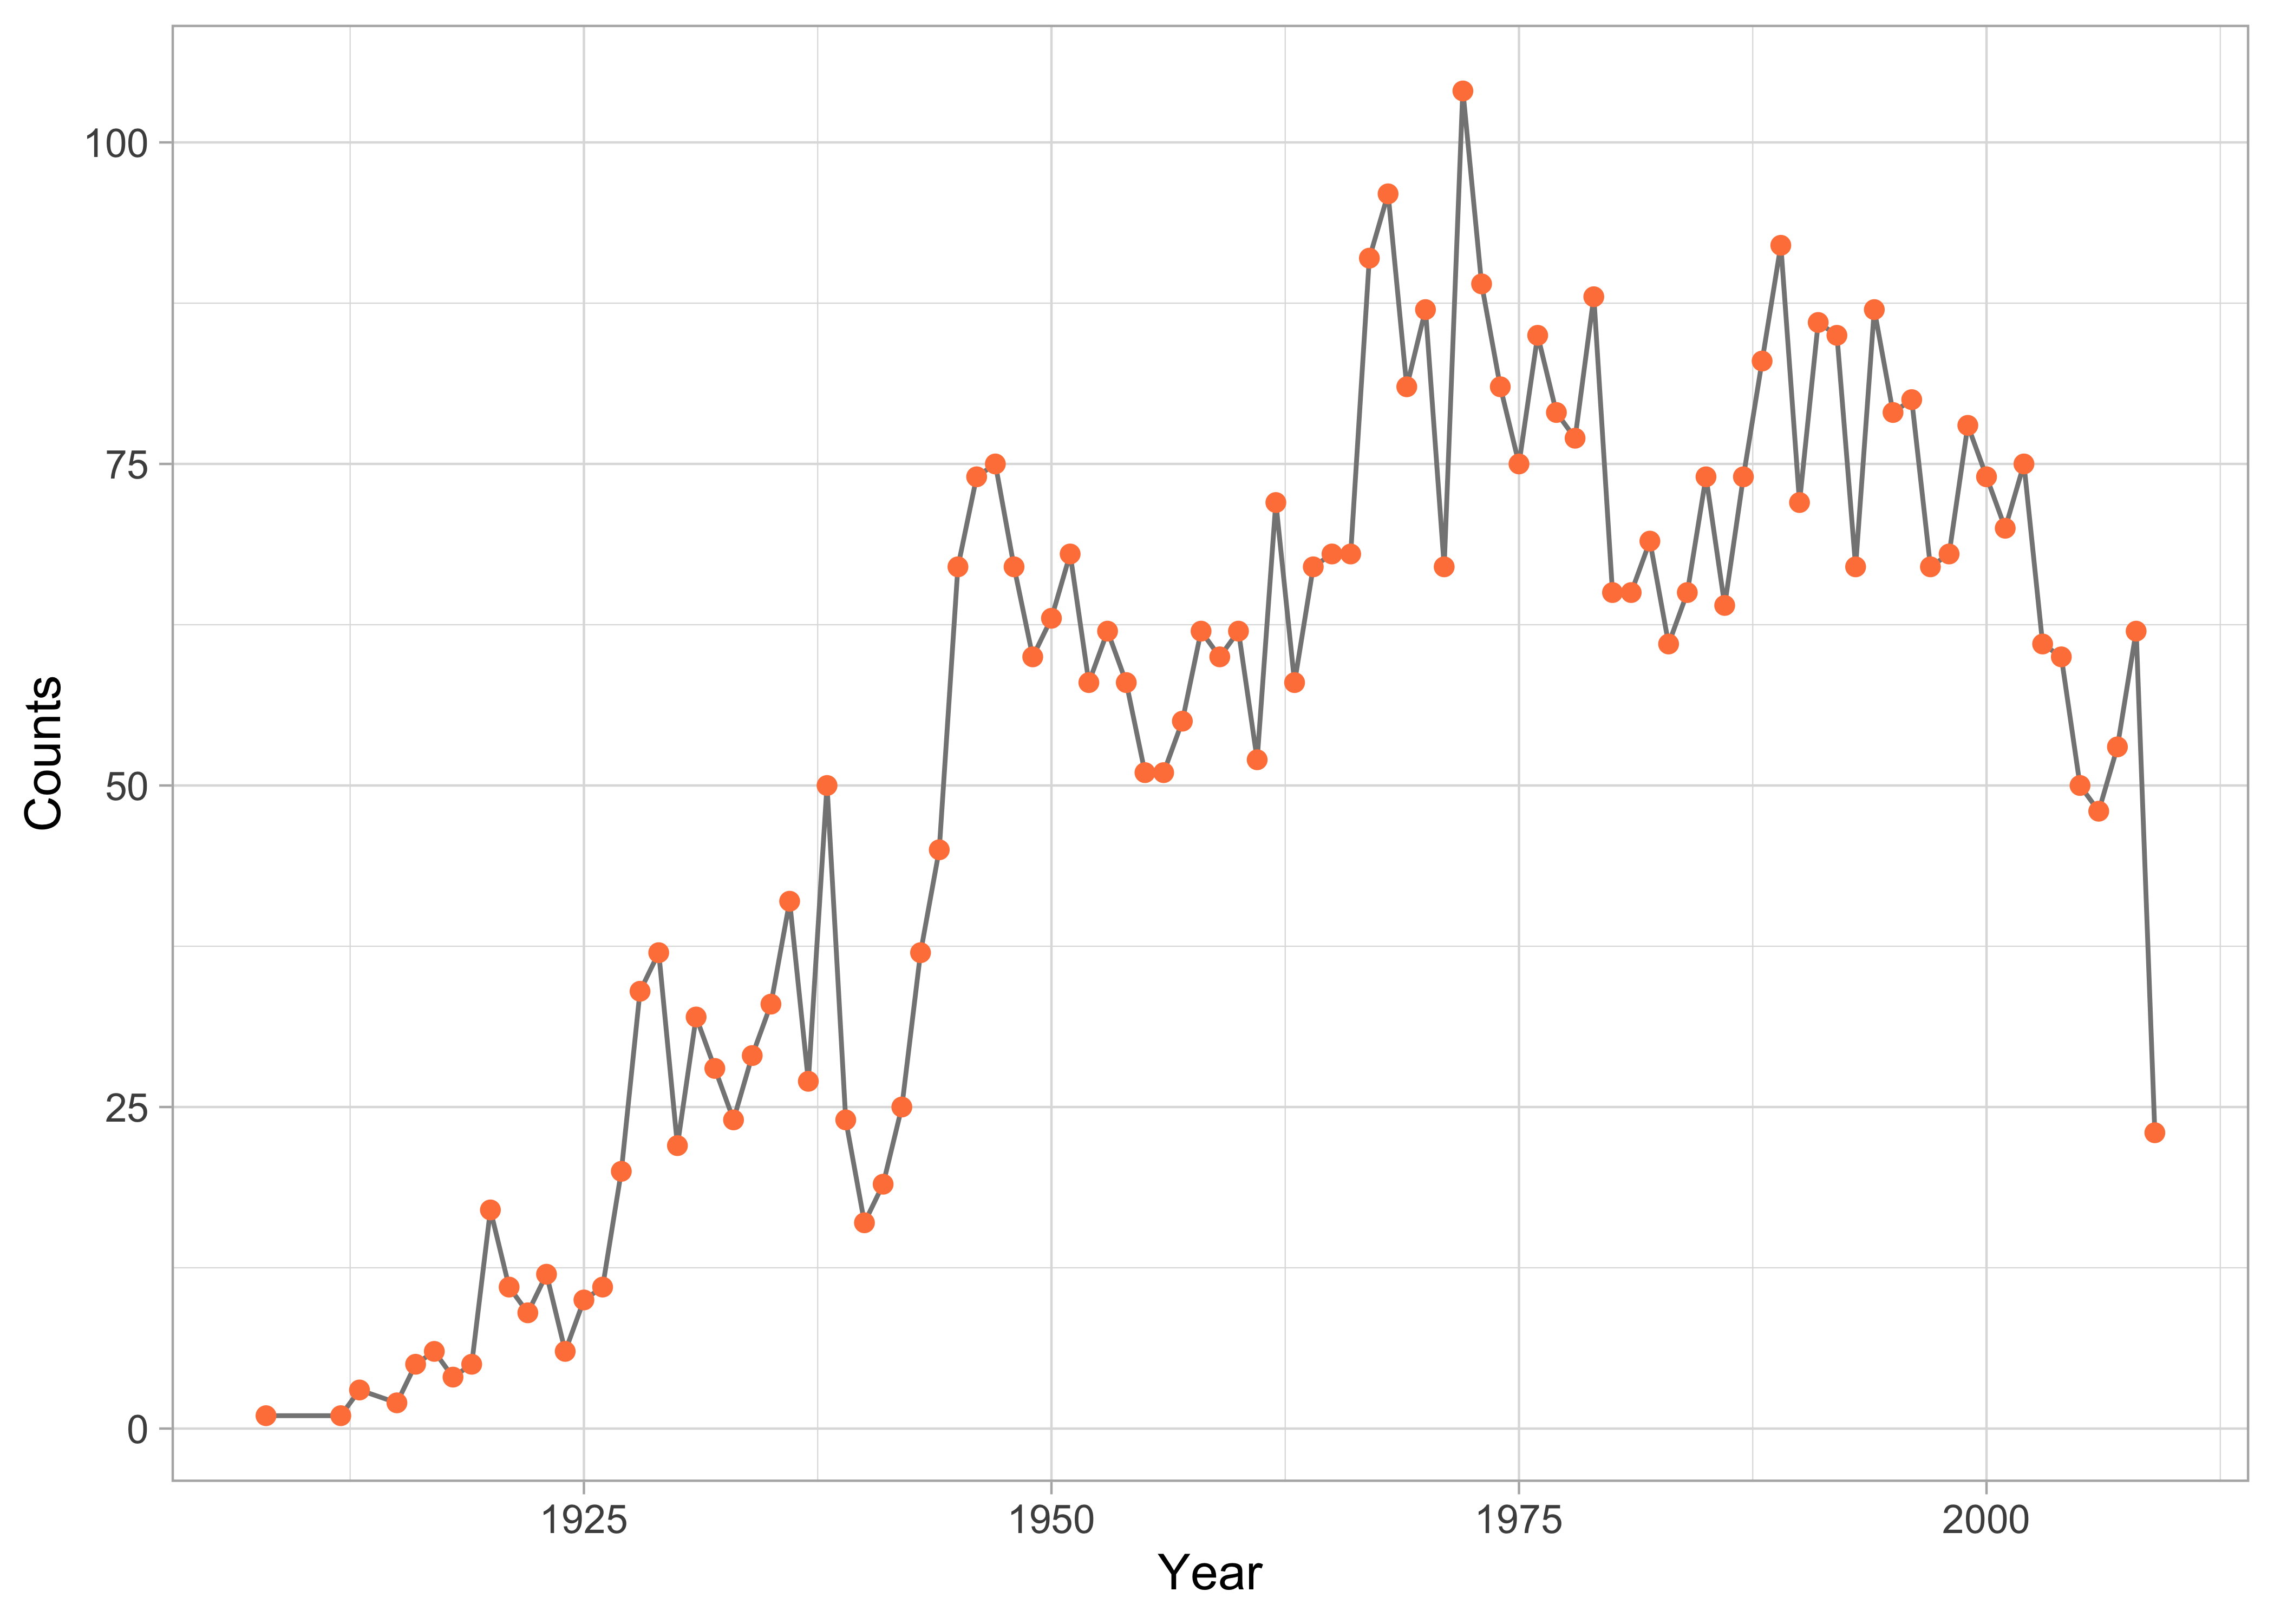
\includegraphics[width=.75\textwidth]{time_flow-1.png}
    \label{fig:time_vs_year}
\end{figure}
The number of air crashes was higher from 1940 to 2005 than before. Next, let’s see if the crash is related to a specific time period. We plot the column chart of air crashes with different scales of time, as shown in Figure \ref{fig:time_vs_counts}. 
\begin{figure}[ht]
    \centering
    \caption{Time V.S. Crashes Counts}
    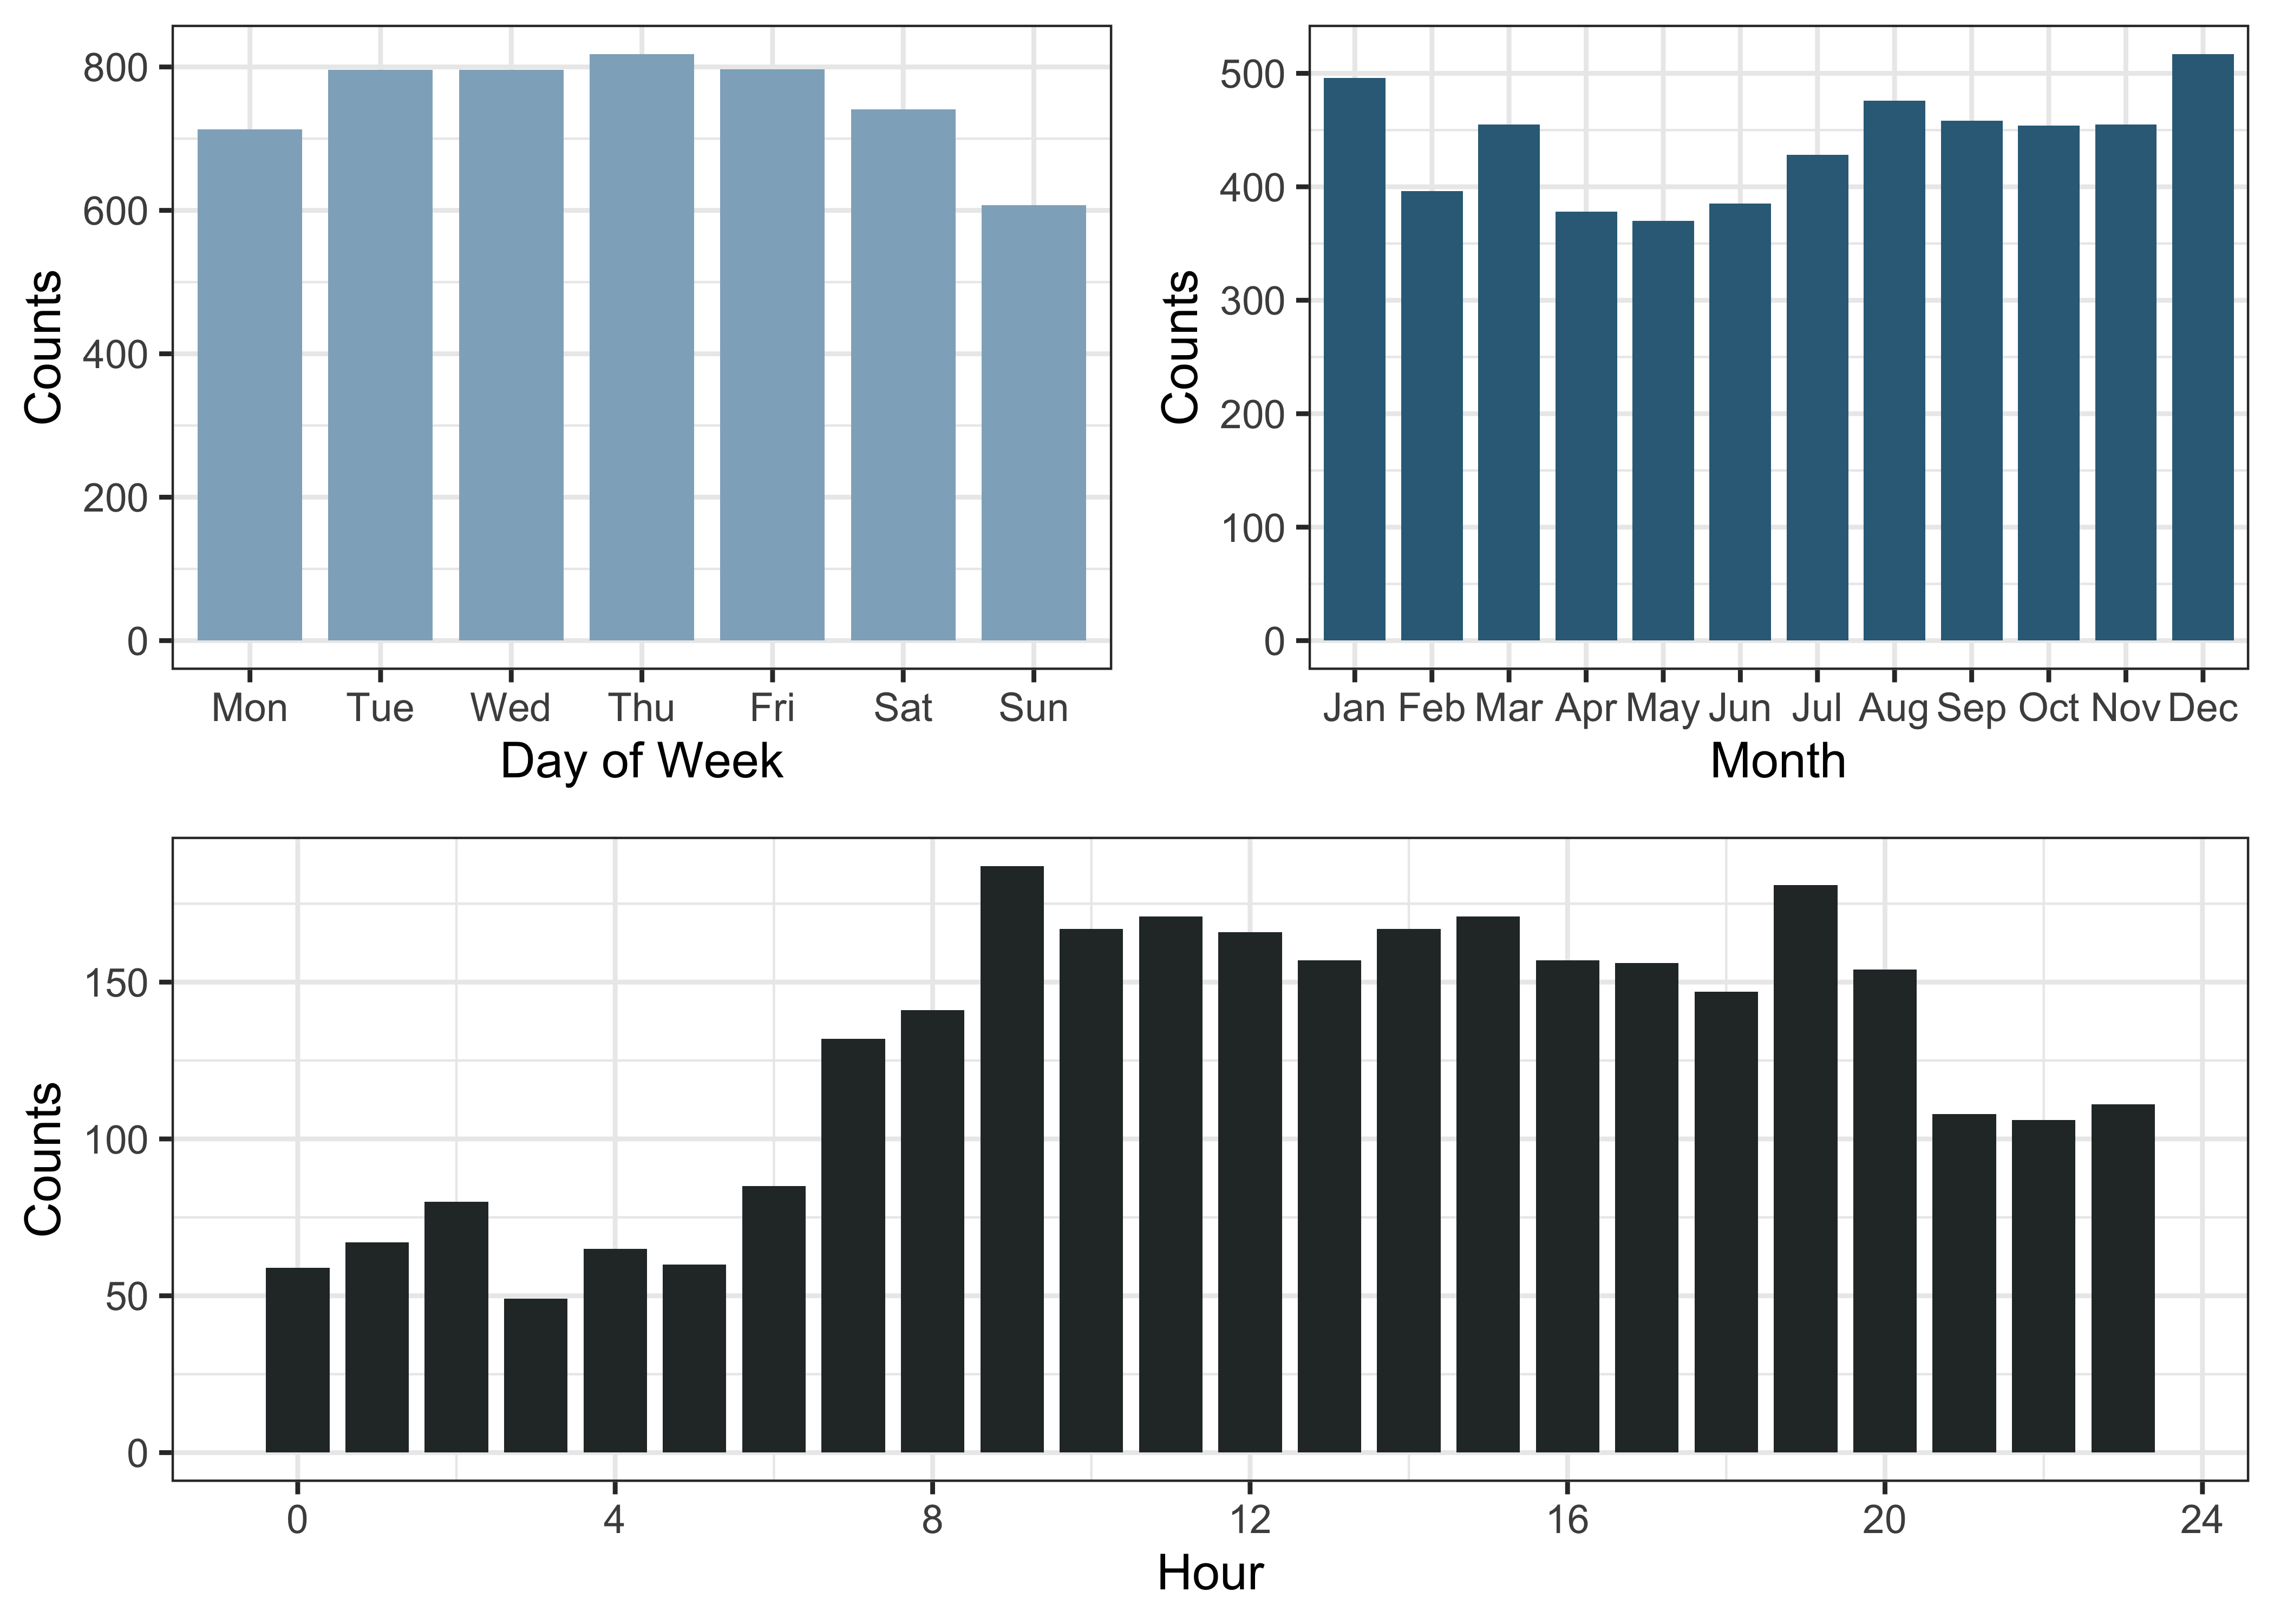
\includegraphics[width=.75\textwidth]{Time_vs_Counts-1.png}
    \label{fig:time_vs_counts}
\end{figure}
A significant increase in the number of air crashes can be seen during certain time periods, like from Wednesday to Friday, January and December, or 7 a.m. to 20 p.m., however, we don’t know the exact reason for this increase. It is possible that some factors during these specific time have led to a higher probability of air crashes. It could also be the total number of flights increased during the specific time period, which led to an increase in the number of crashes. 

We also explored the relationship between survival rate and time. Figure \ref{fig:time_vs_surrate}
\begin{figure}[ht]
    \centering
    \caption{Time V.S. Survival Rate}
    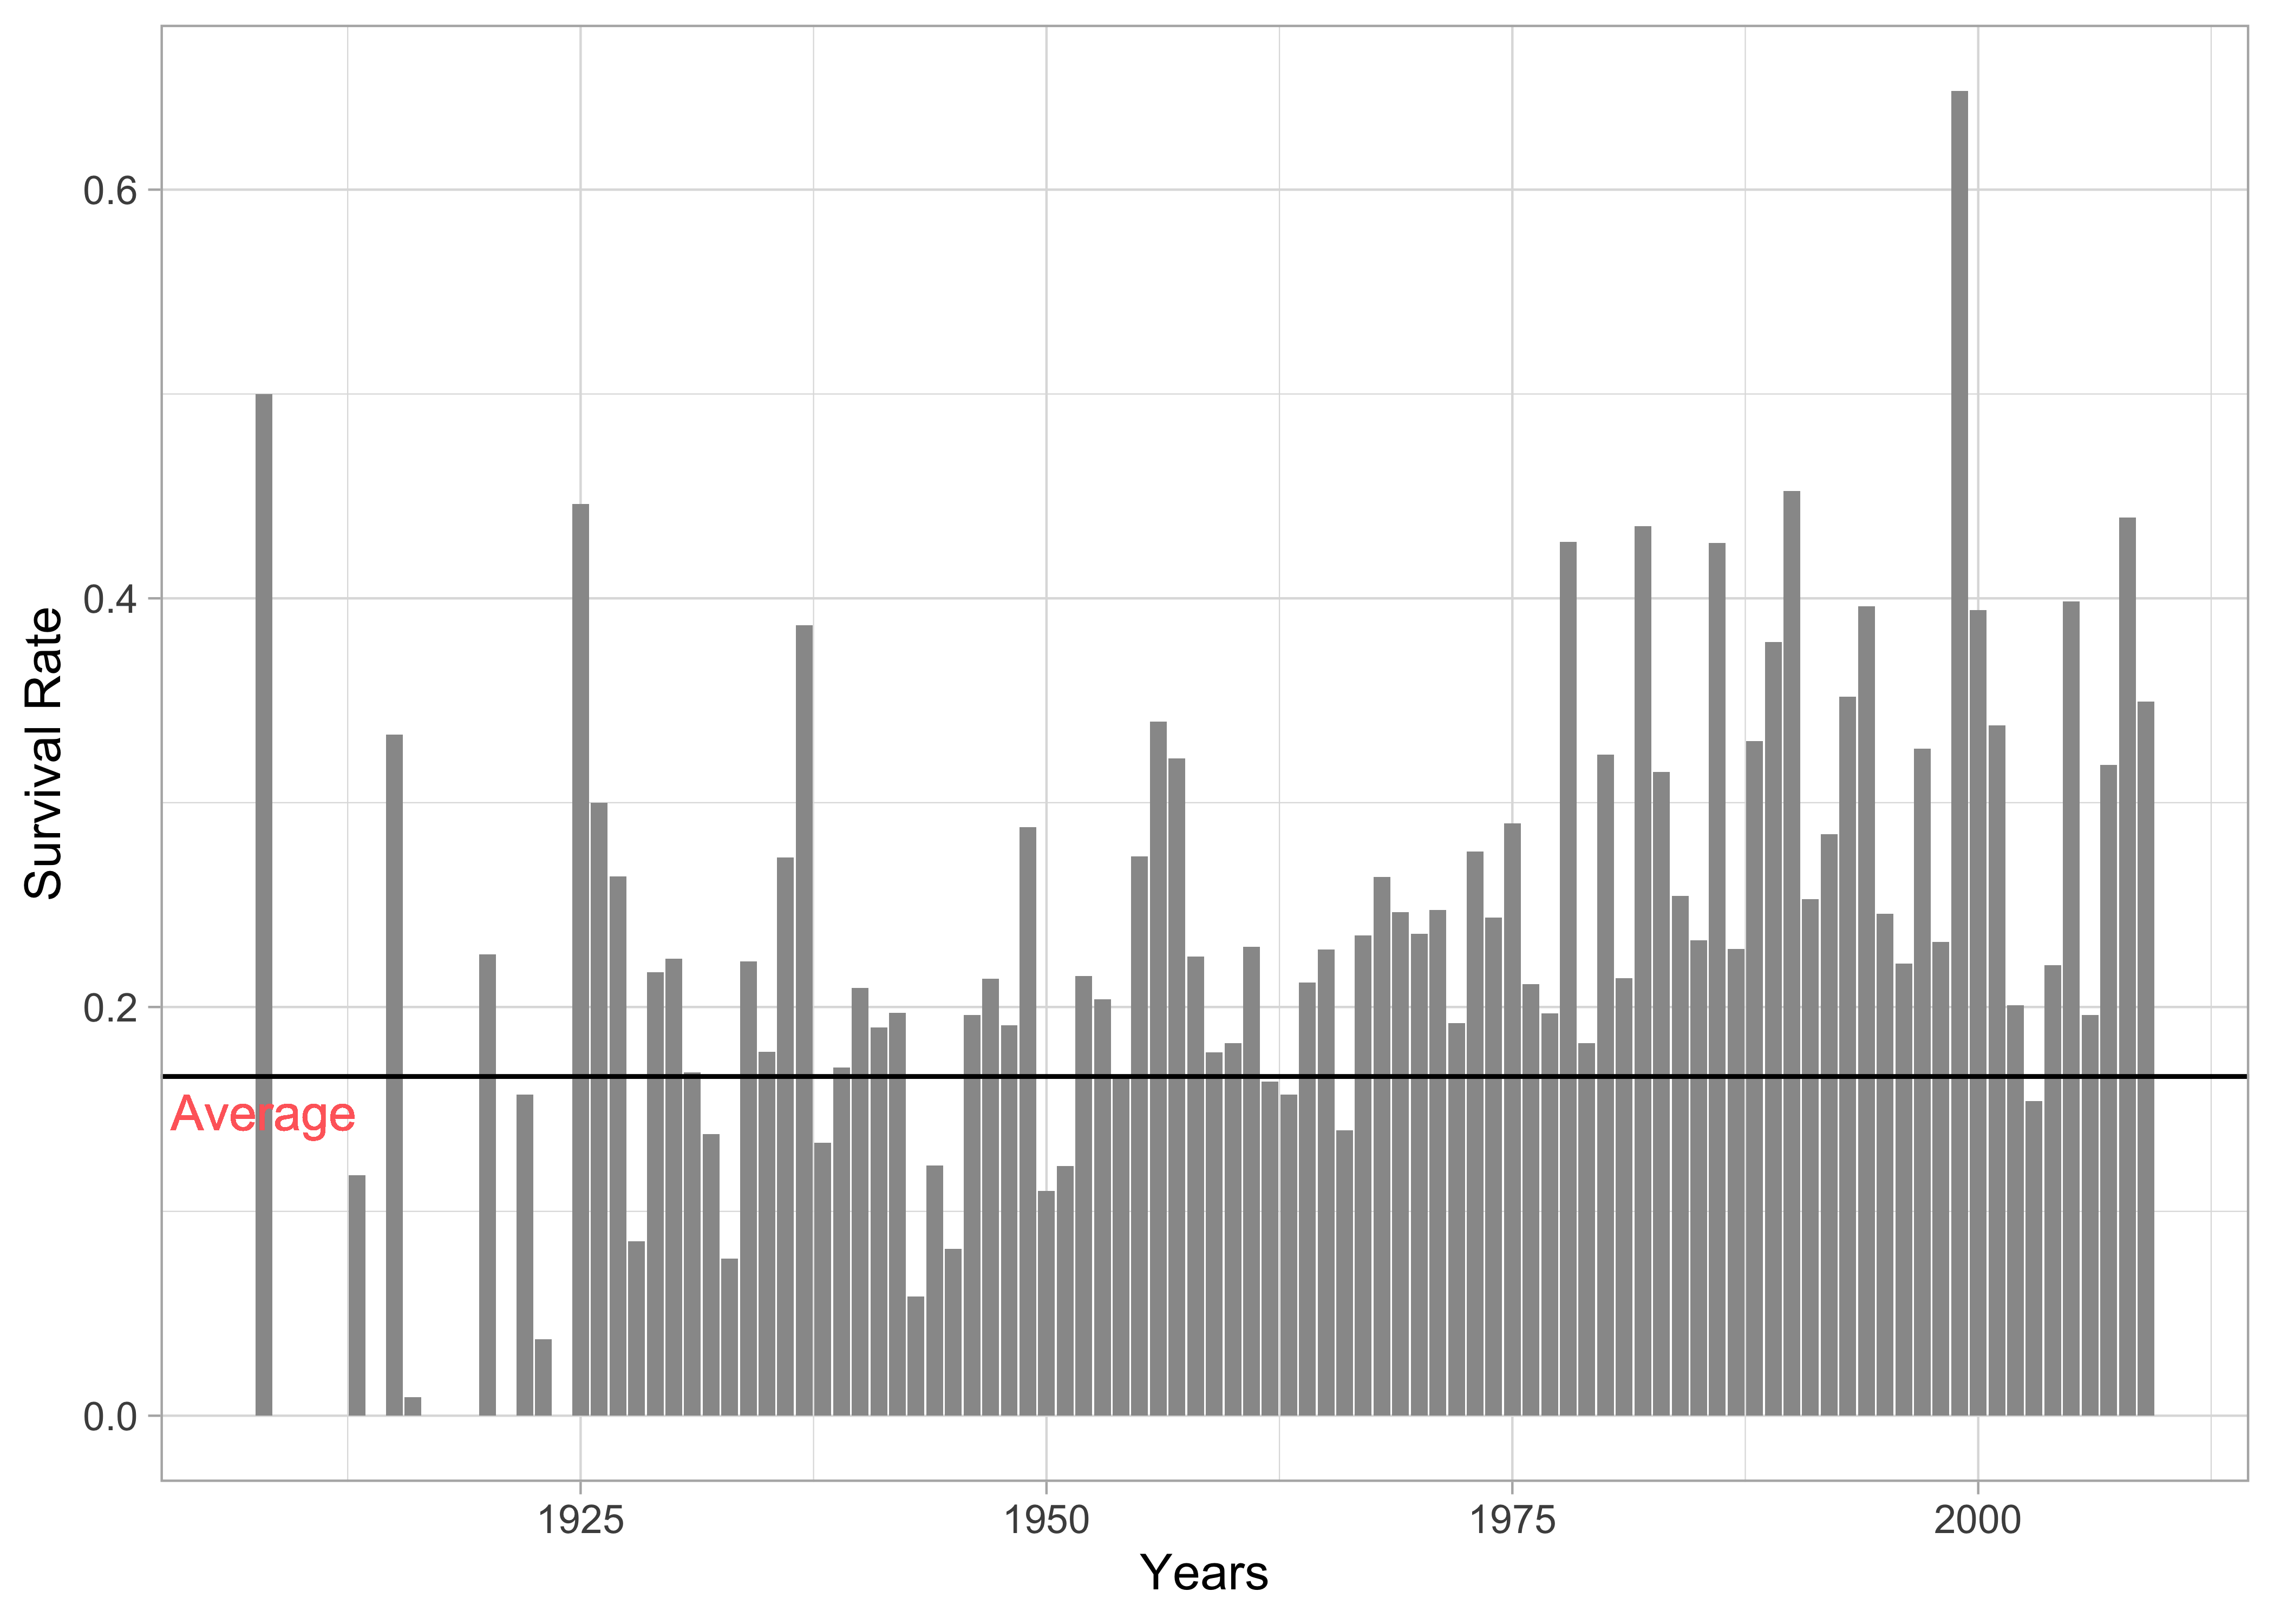
\includegraphics[width=.75\textwidth]{time_vs_surrate-1.png}
    \label{fig:time_vs_surrate}
\end{figure}
shows the average survival rate per year. As we can see, the survival rates steadily increased from the late 1960's to peak in the late 1990's. The majority of years before 1975 have overall survival rates below $20\%$. Since 1975 there have only been four years where the overall survival rate dropped below $20\%$. This change may be related to the fact that both manufacturers and pilots are taking aviation safety more seriously. 

\subsection{Cluster Analysis}

K-means clustering is an unsupervised machine learning algorithm that aims to partition observations into clusters in which each observation belongs to the cluster with the nearest mean. We first compare the results for $k= 2, 3, 4, 5$. They are shown as Figure \ref{fig:cluster_result}. 
\begin{figure}[ht]
    \centering
    \caption{K-means results}
    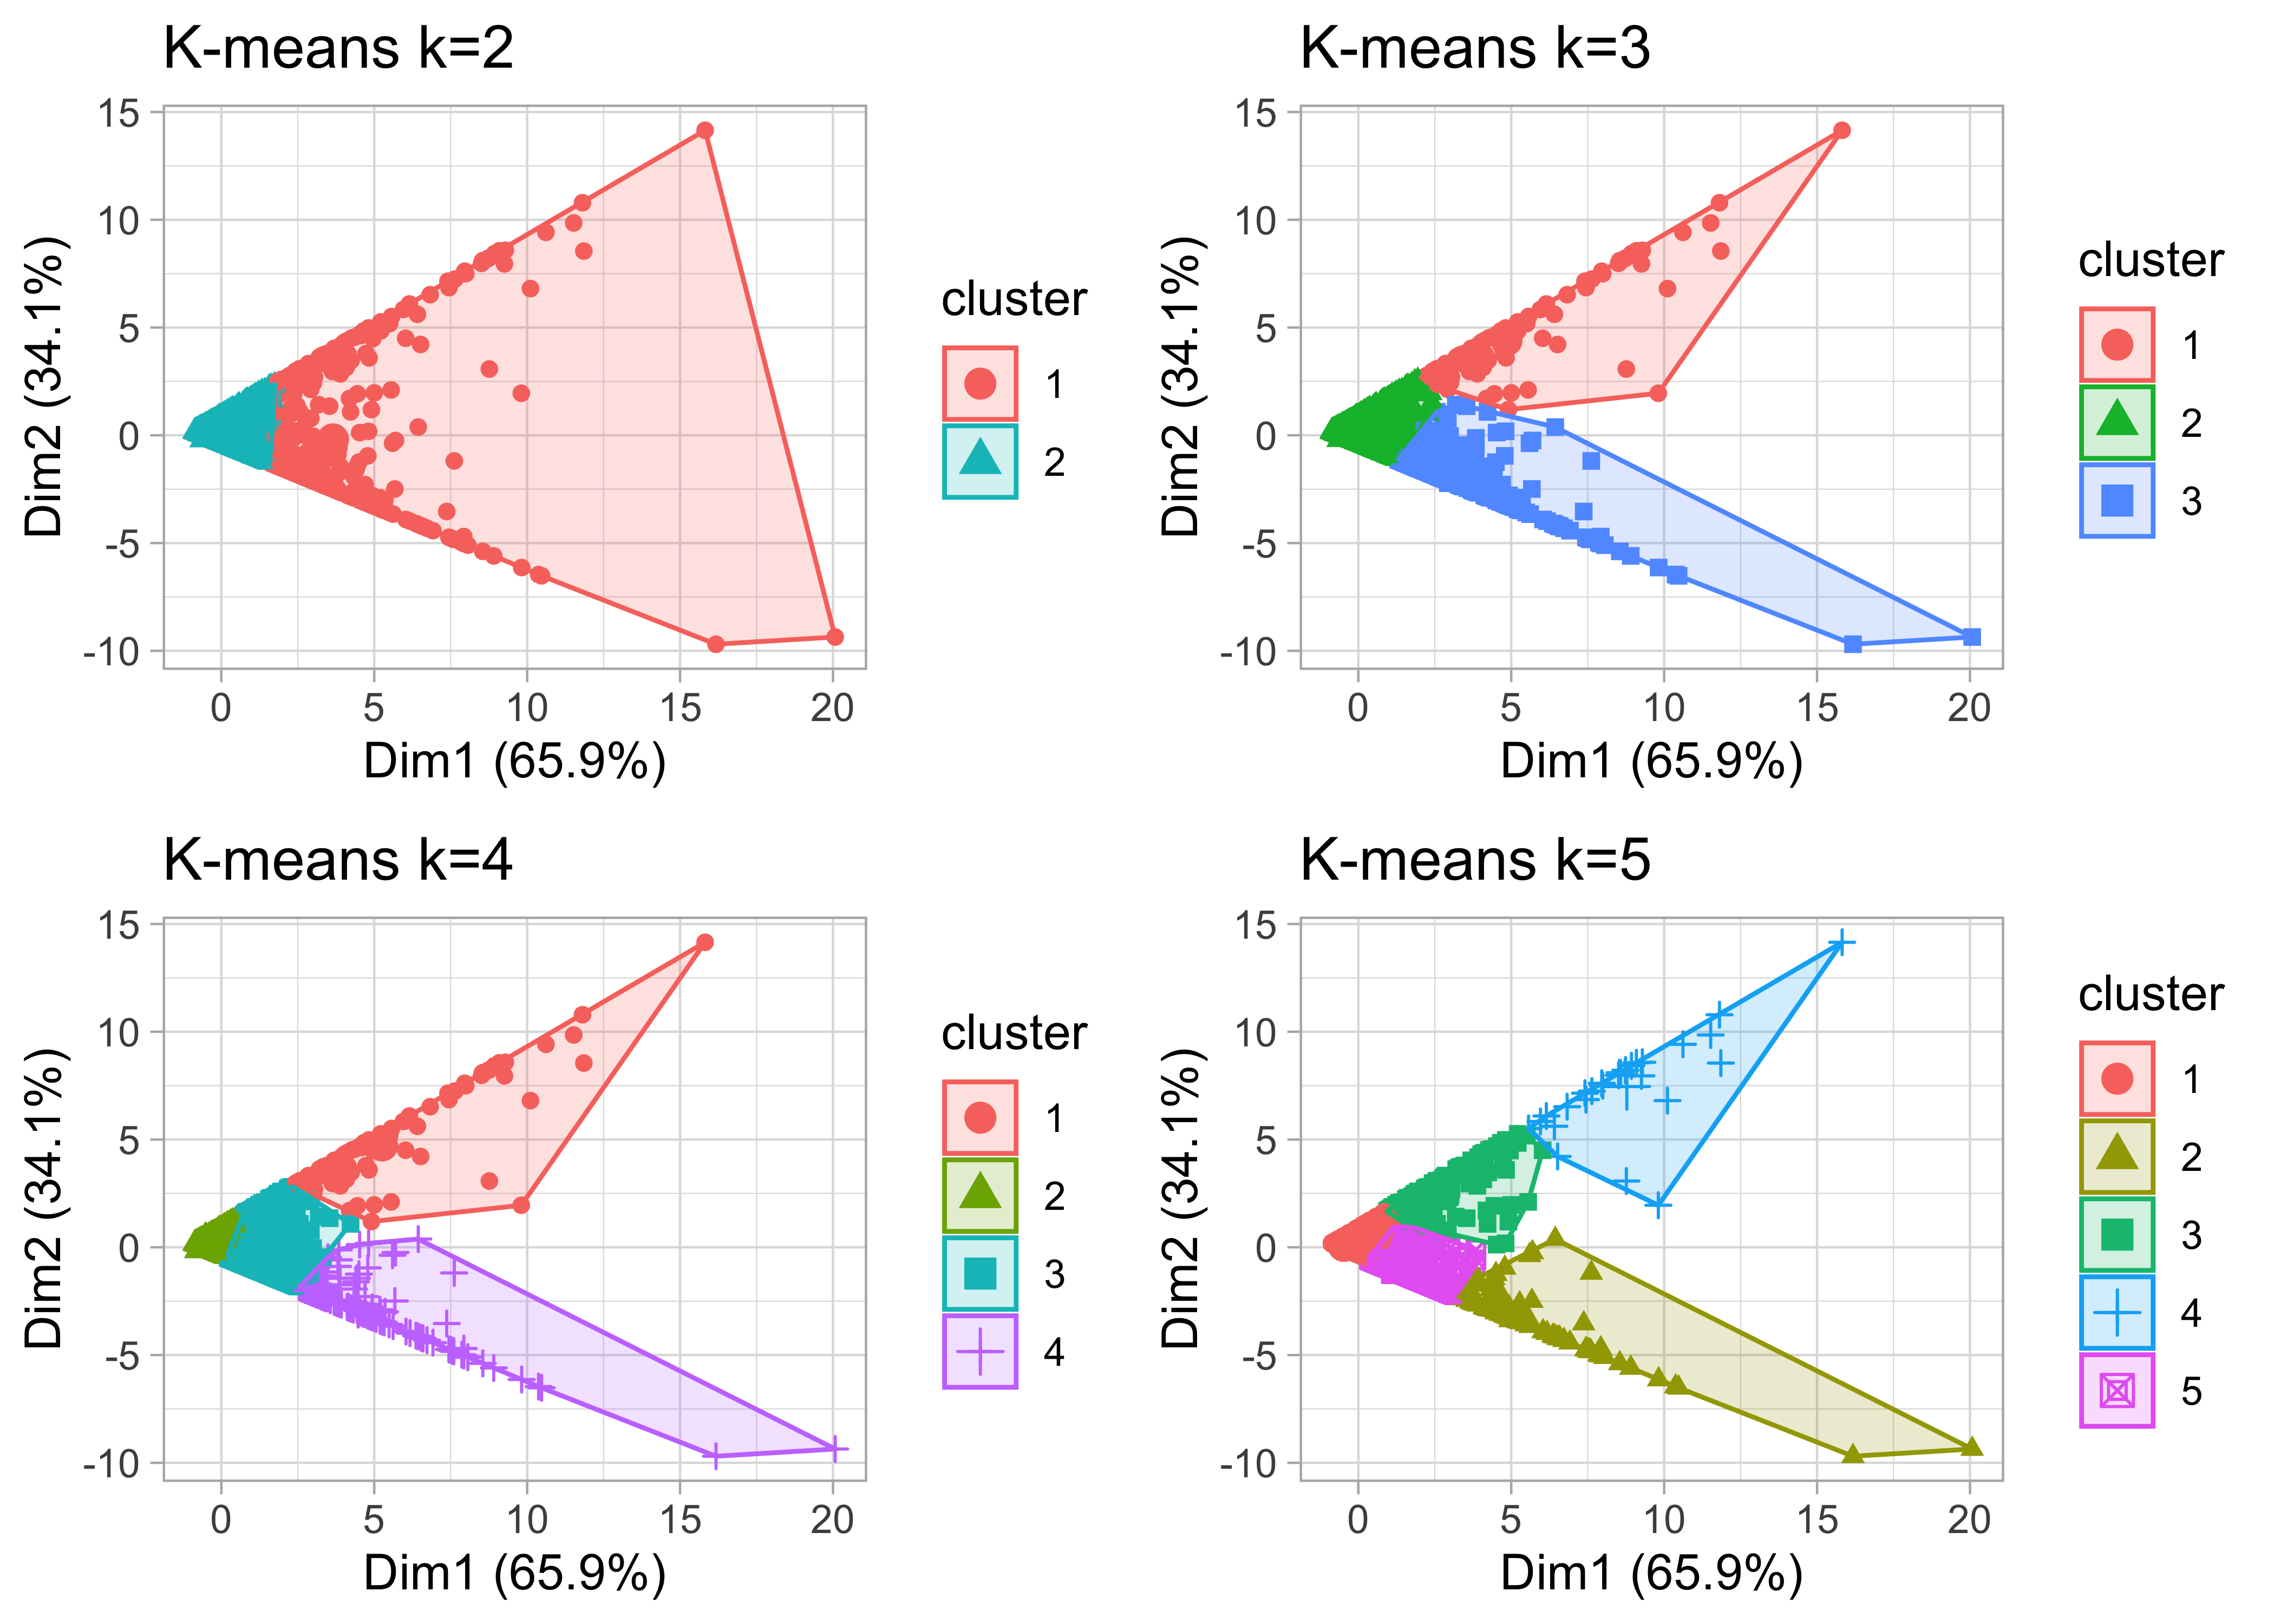
\includegraphics[width=.75\textwidth]{k-means results-1.png}
    \label{fig:cluster_result}
\end{figure}
We can see that the results are similar for different K values, so it is difficult to determine the appropriate K value. Therefore, we plot the ELBOW plot about the total within sum of squares of the errors. As shown in the Figure \ref{fig:elbow},
\begin{figure}[ht]
    \centering
    \caption{Optimal number of the clusters}
    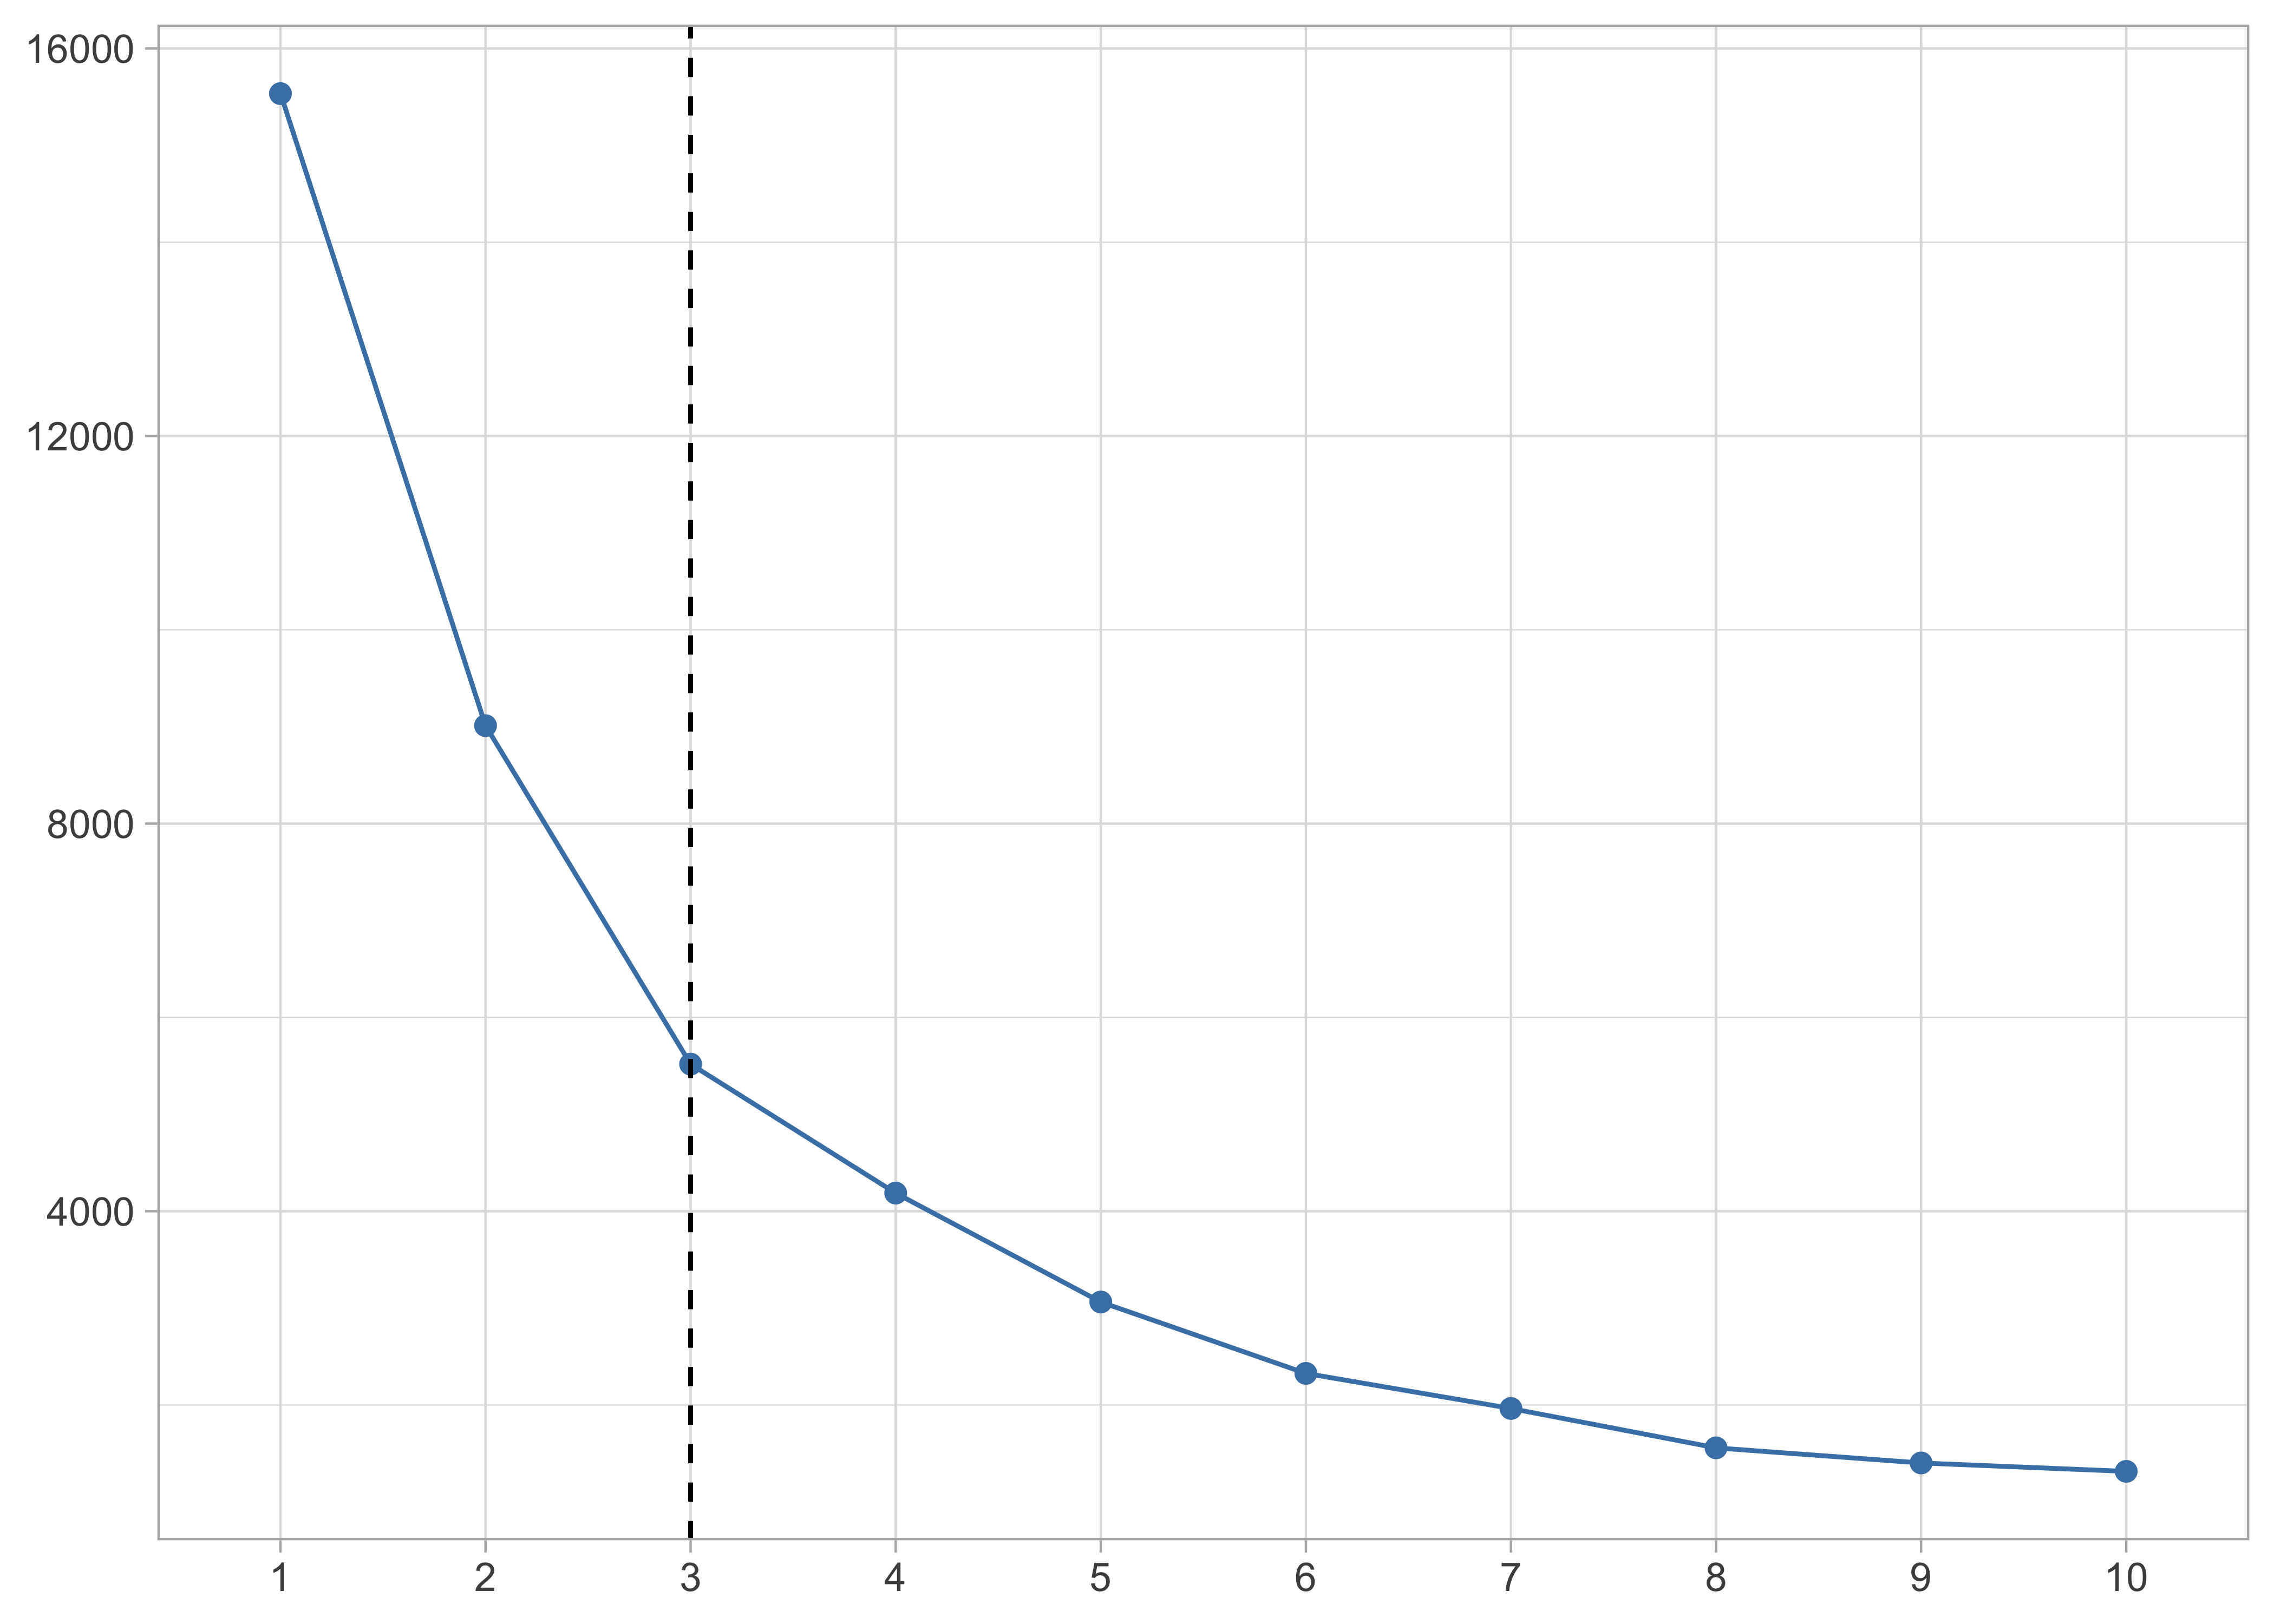
\includegraphics[width=.75\textwidth]{elbow-1.png}
    \label{fig:elbow}
\end{figure}
the decrease in the error sum of squares is not significant after $3$, so we choose $k=3$. 

After that, in order to see if there is a significant difference between the different clusters, we calculate mean values of the \emph{Aboard}, \emph{Fatalities} and \emph{Survival Rate} for each cluster, and the results are shown in Table \ref{tab:comparison}. 
\begin{table}[ht]
\centering
\caption{Comparison for different clusters}
\label{tab:comparison}
\small
\begin{tabular}{ccccc}
\hline
\textbf{Cluster} & \textbf{Counts} & \textbf{Mean Aboard} & \textbf{Mean Fatalities} & \textbf{Mean Survival Rate} \\ \hline
1 & 111  & 177.65766 & 12.71171  & 0.93048094 \\
2 & 4723 & 17.15266  & 13.26064  & 0.15623132 \\
3 & 345  & 124.80870 & 117.78261 & 0.05316435 \\ \hline
\end{tabular}
\end{table}
By comparing the different values, we can find that the clustering results are quite good. We can clearly distinguish the features of each cluster by the survival rate. And each cluster describes a situation of an air crash. 
\begin{itemize}
    \item Cluster 1: Air crashes with a high survival rate $93.05\%$; 
    \item Cluster 2: Air crashes with an average survival rate $15.62\%$; 
    \item Cluster 3: Air crashes a low survival rate $5.32\%$. 
\end{itemize}
The survival rates for Cluster $2$ was close to the mean survival rate of $16.5\%$. Cluster $2$ makes up more than $90\%$ of the total data with $4723$ crashes. Clusters $1$ and $2$ both are larger passenger planes with a huge difference in mean survival rates. And there were three times as many large passenger planes that had a low mean survival rate v.s. a high mean survival rate. Therefore, these three clusters can represent the following specific flights: 
\begin{itemize}
    \item Cluster 1: Large Passenger High Survival; 
    \item Cluster 2: Small-Midsize Crashes; 
    \item Cluster 3: Large Passenger High Fatality. 
\end{itemize}

\subsection{Type, Operator and Survival Rate}
It can be noted that the crashes with high survival rates and high fatality rates are all large planes with a large number of passengers. But why is there such a big difference in survival rates for the same large planes? The type of plane and operator may play a decisive role. 

The top 10 models with the highest mortality and survival rates are shown in Figures \ref{fig:Type10}.

\begin{figure}[htp]
    \centering
    \caption{Top 10 Large Passenger High Survival(Fatality) Crashes by Model}
    \label{fig:Type10}
    \subfigure{
    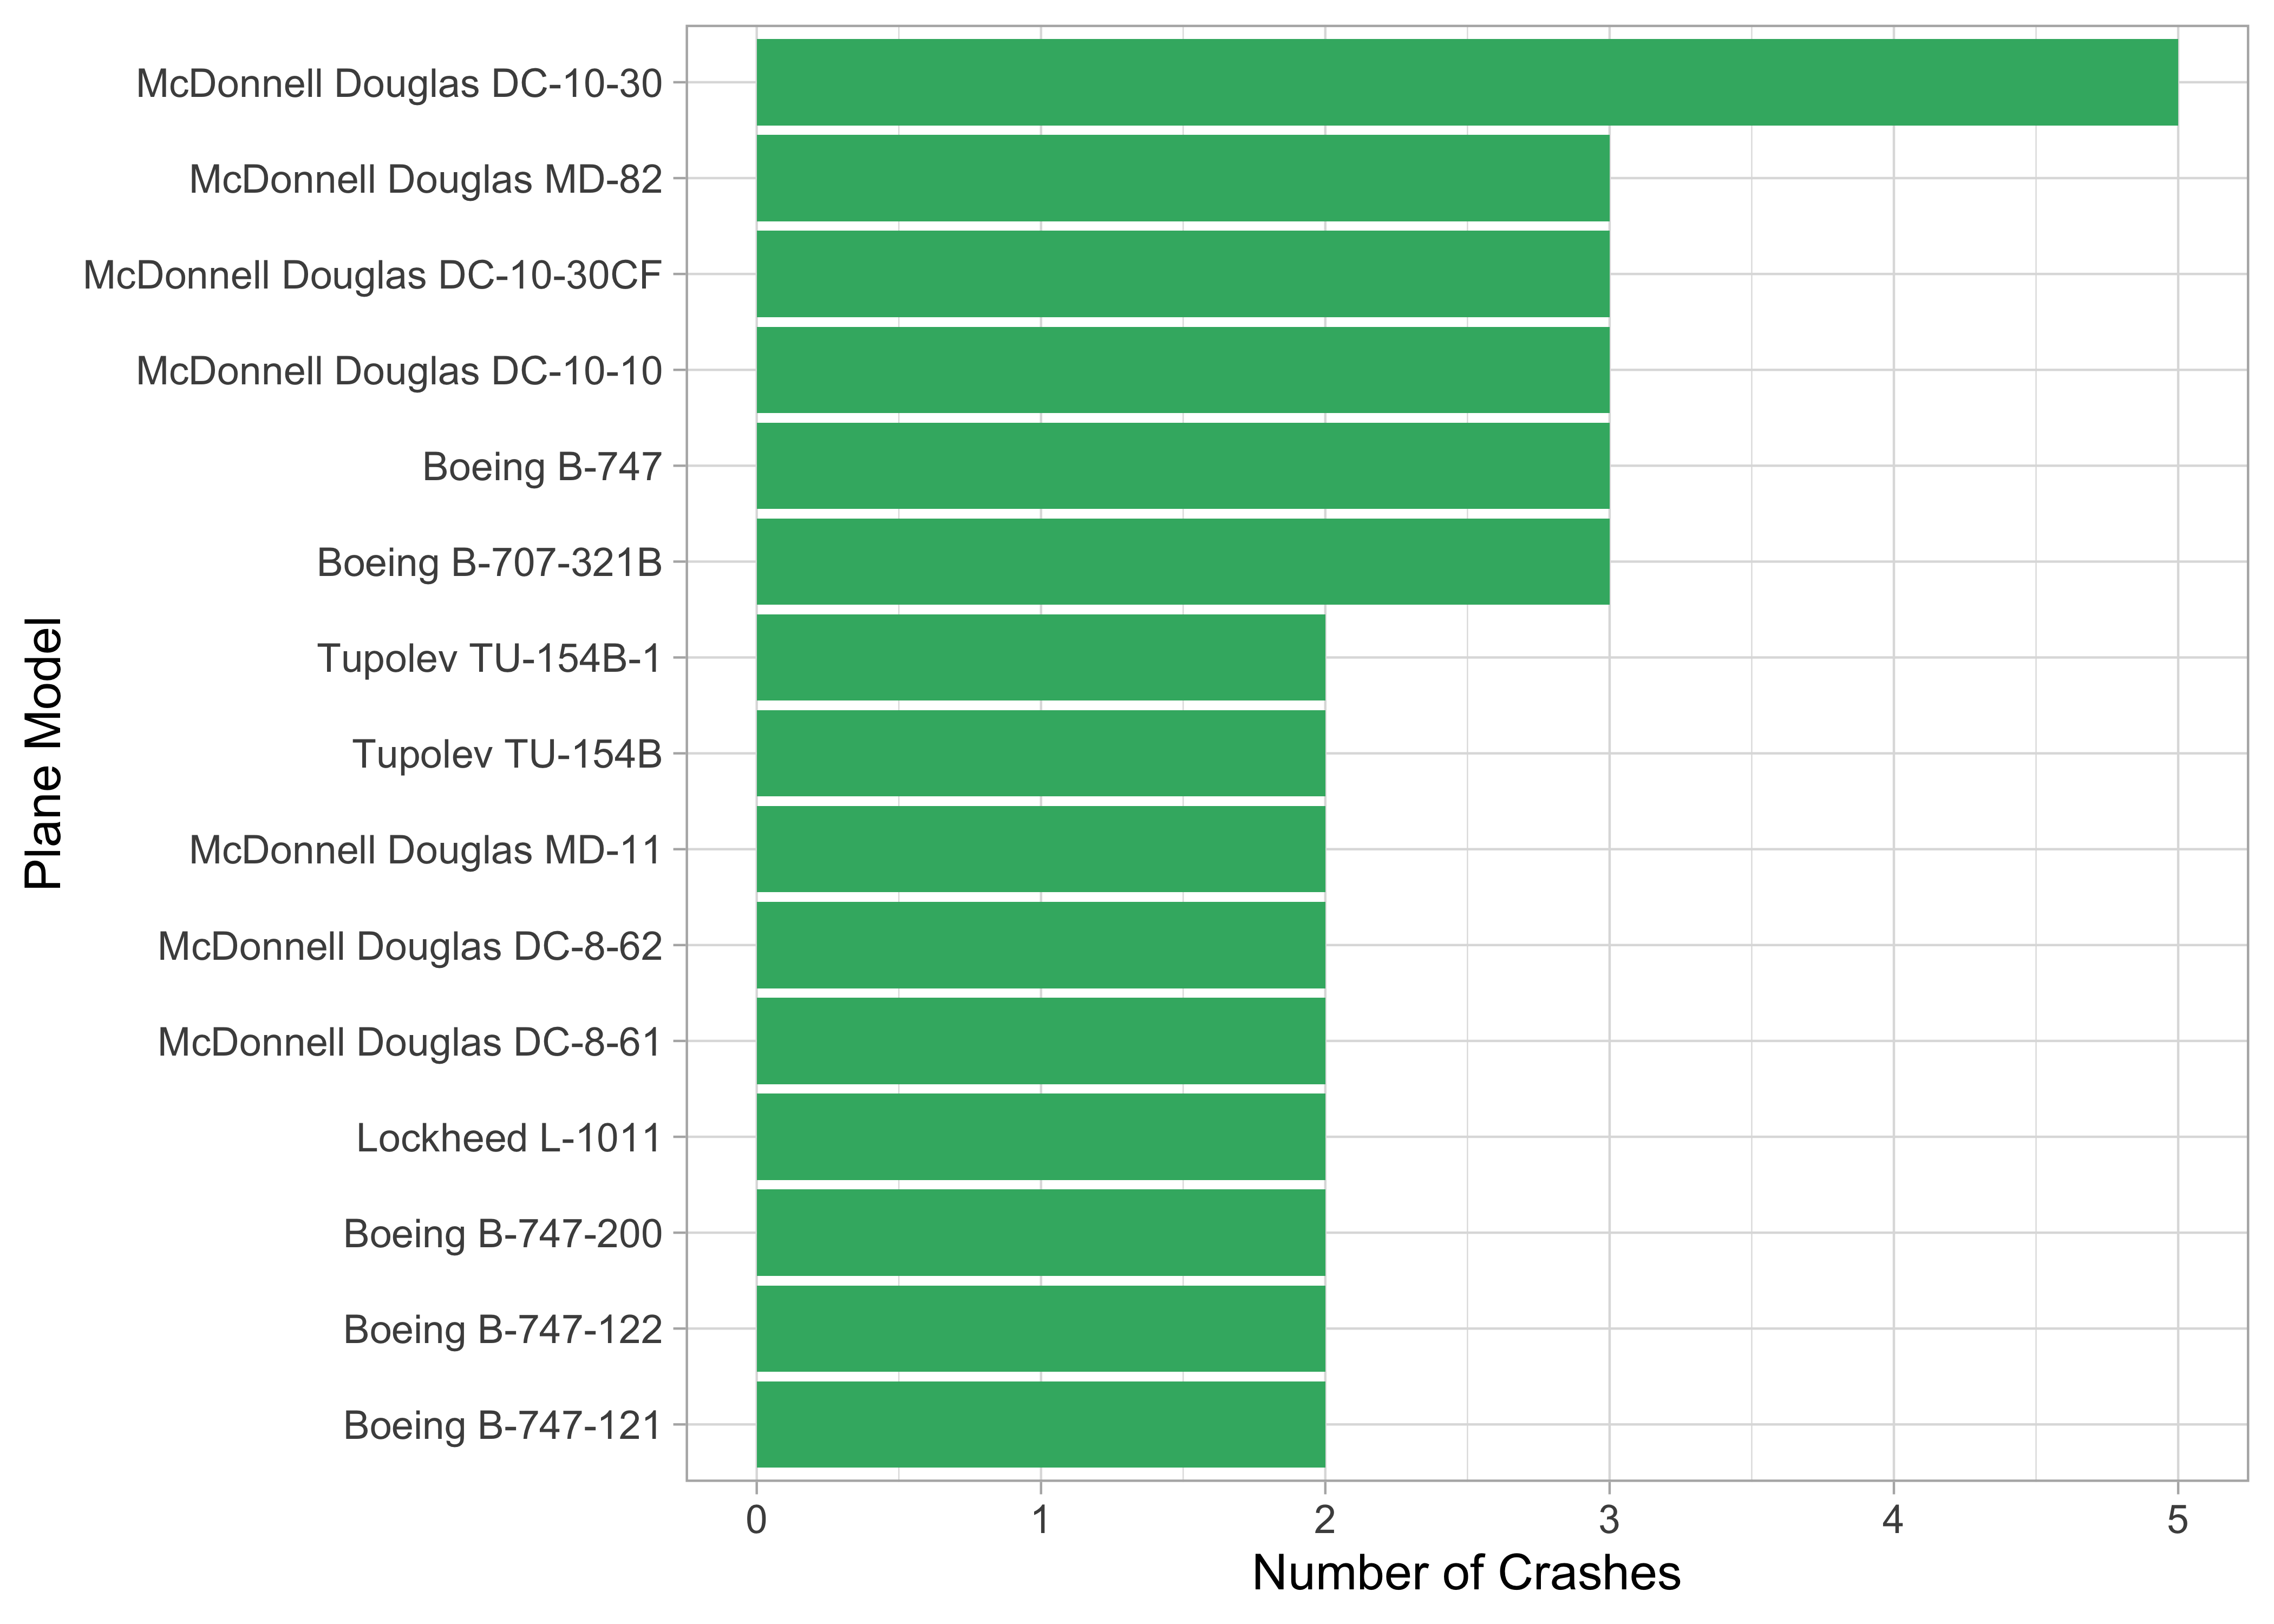
\includegraphics[width=0.46\textwidth]{Type10_1-1.png}}
    \subfigure{
    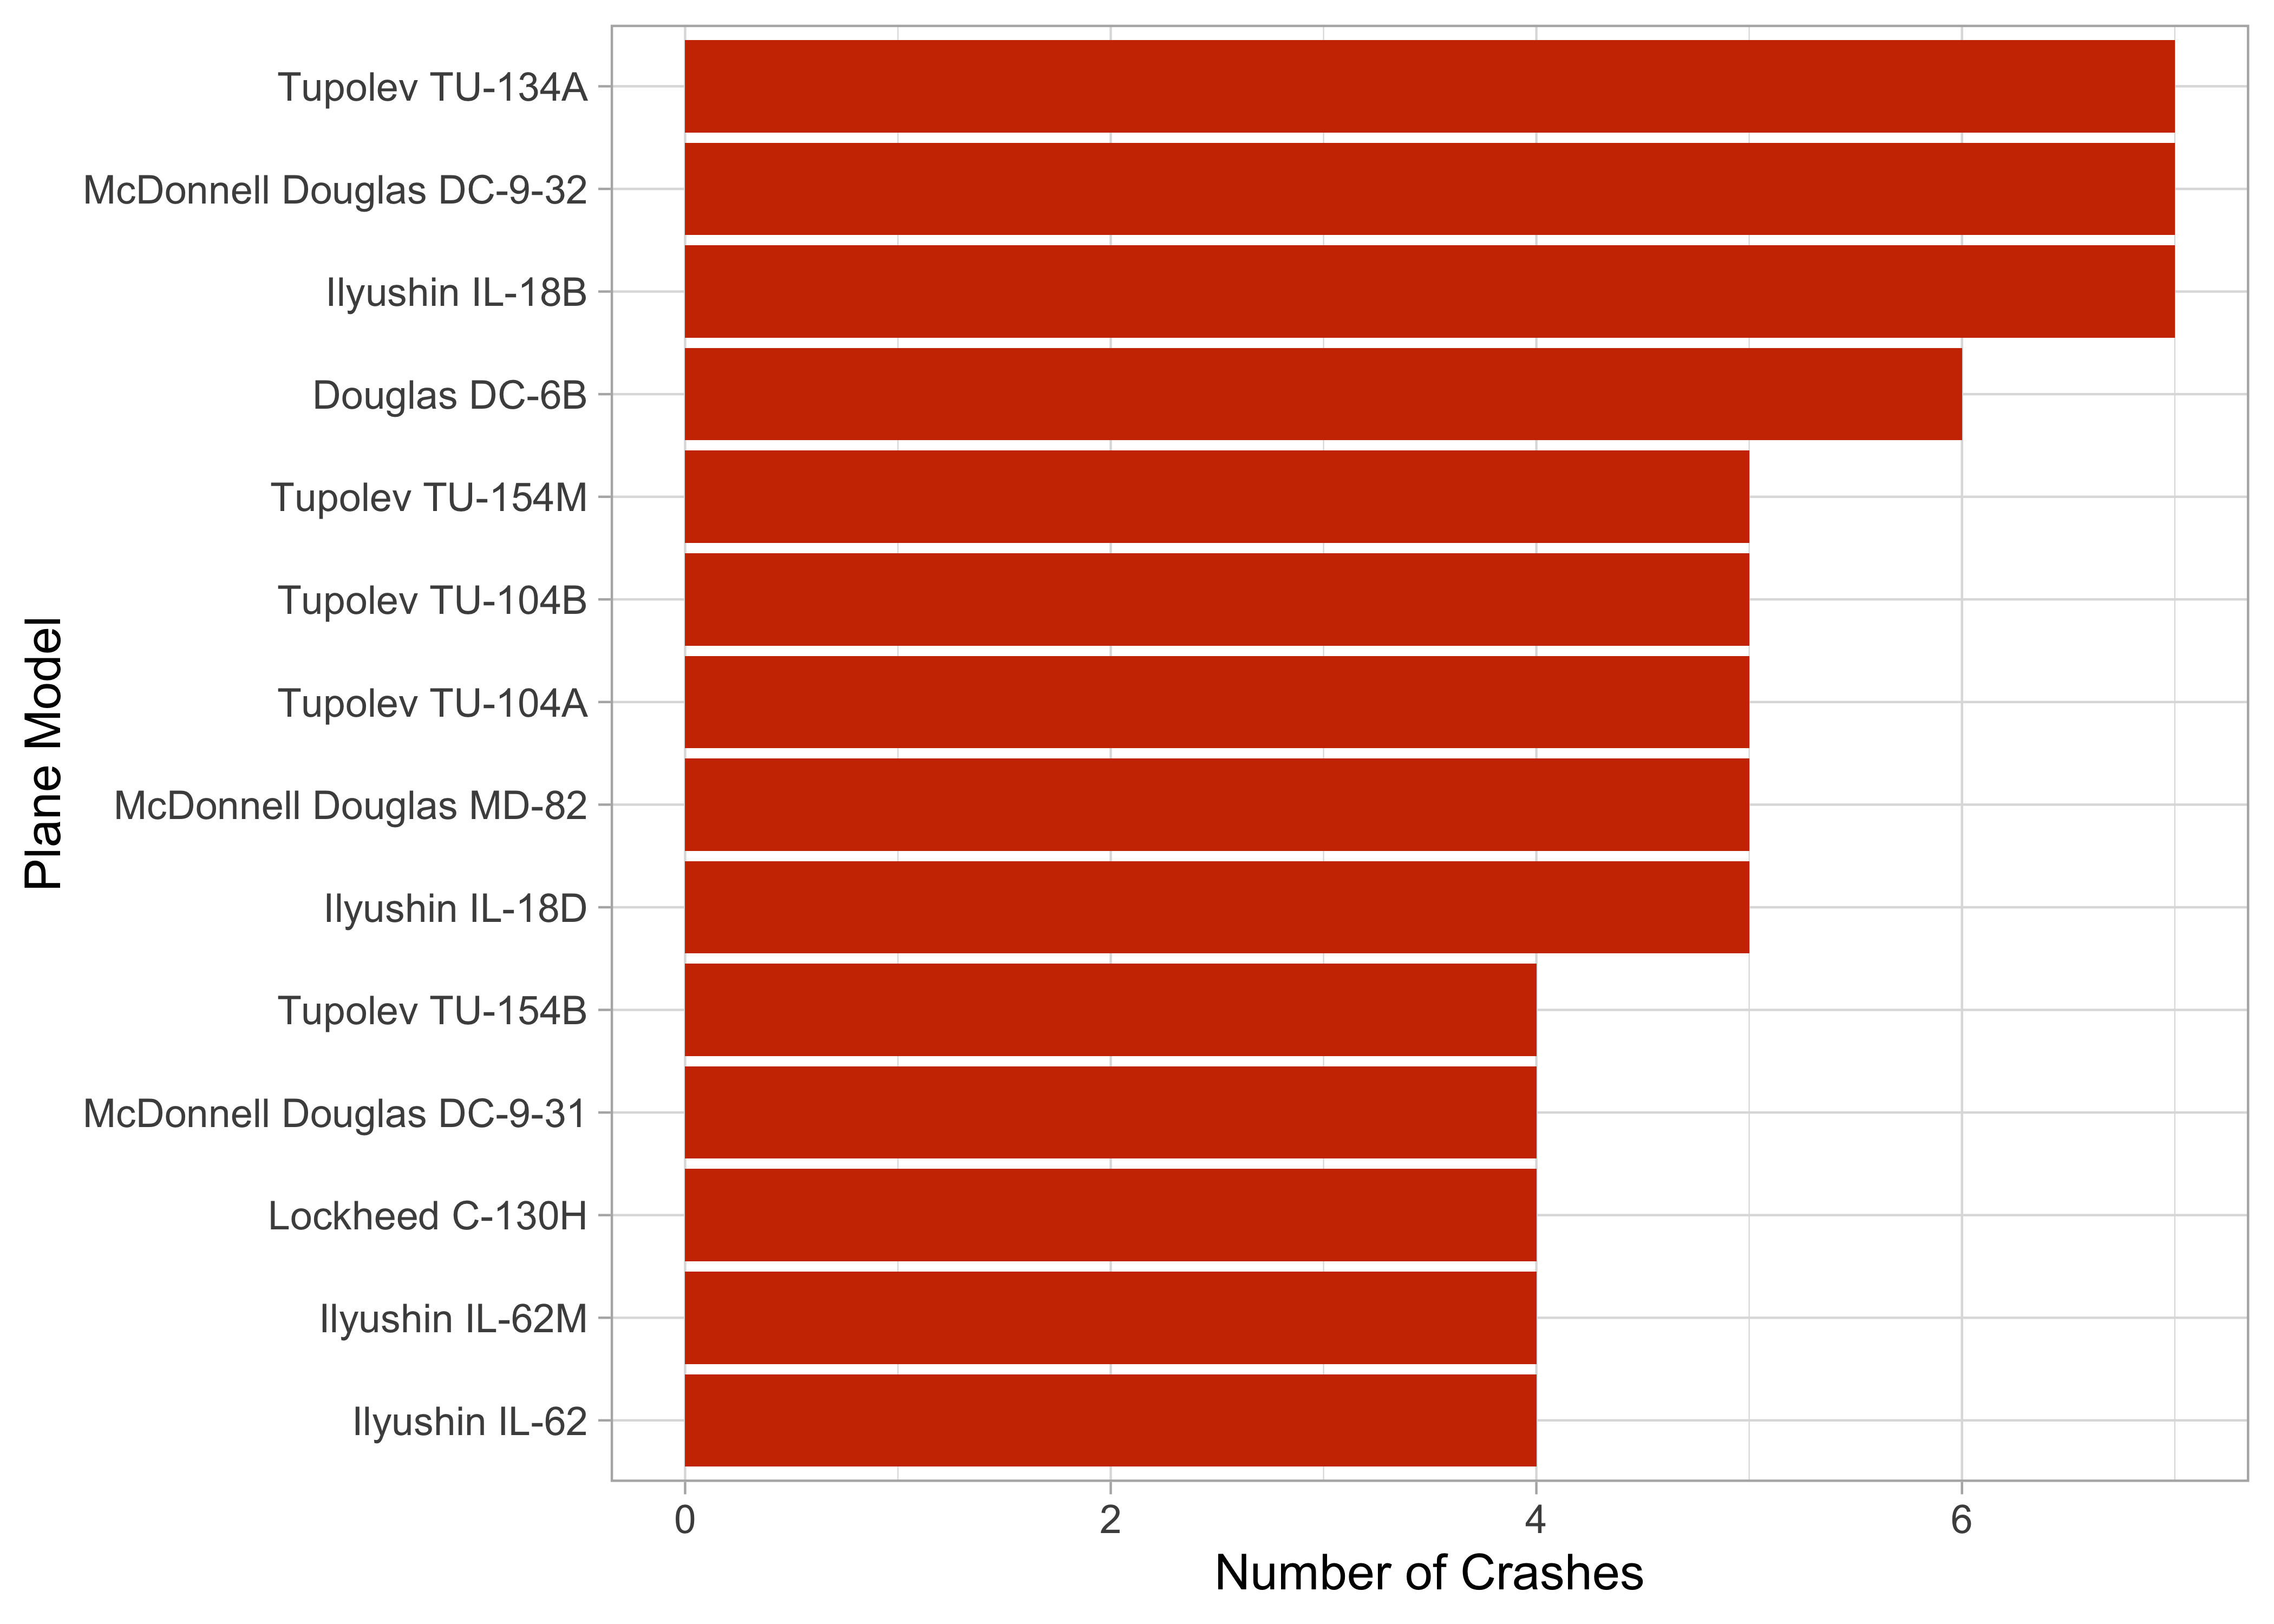
\includegraphics[width=0.46\textwidth]{Type10_2-1.png}}
\end{figure}
From the plot we can see the following two points: 
\begin{itemize}
    \item American \emph{McDonnell Douglas DC} and \emph{Boeing} 747 models appeared most frequently among the top 10 large passenger plane crashes with high survival rates. 
    \item American \emph{McDonnell Douglas DC} models and the Russian \emph{Tupolev} and \emph{Ilyushin} models made up the top 10 large passenger plane crashes with high fatalities. 
\end{itemize}

Similarly, the top 10 operator in terms of survival and mortality rates are shown in Figure \ref{fig:Op10}. 
\begin{figure}[htp]
    \centering
    \caption{Top 10 Large Passenger High Survival(Fatality) Crashes by Operator}
    \label{fig:Op10}
    \subfigure{
    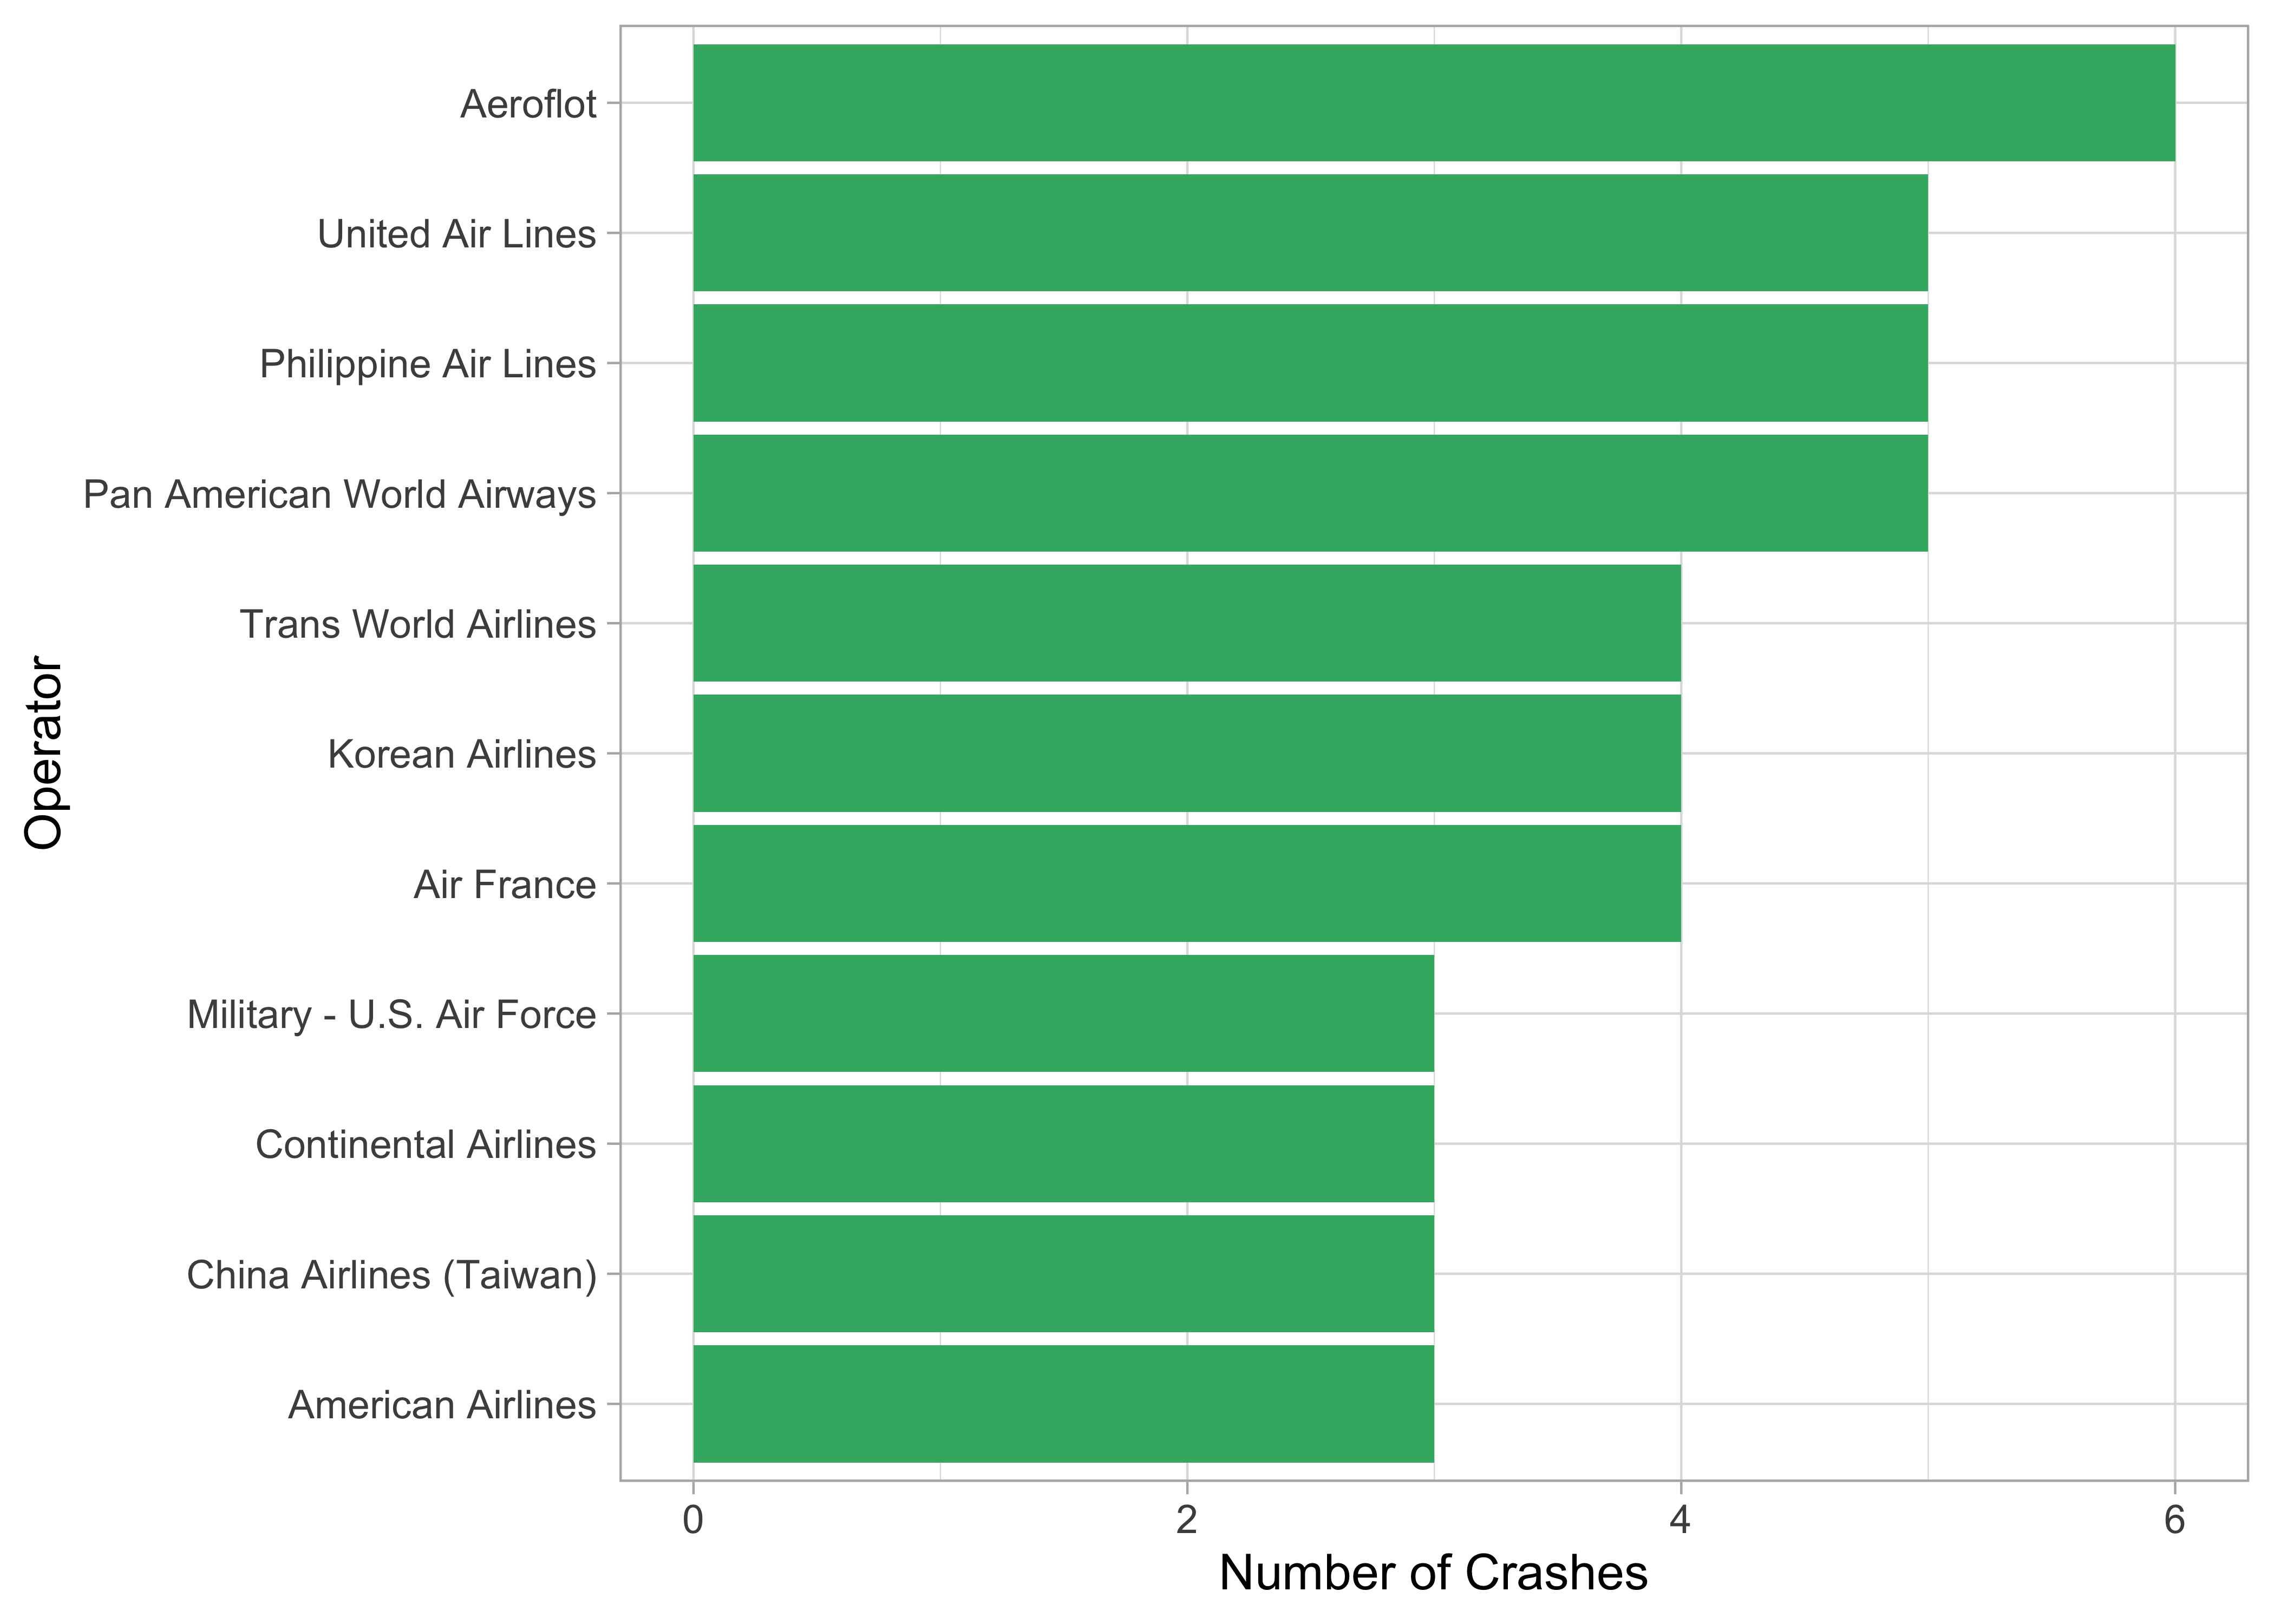
\includegraphics[width=0.46\textwidth]{Op1-1.png}}
    \subfigure{
    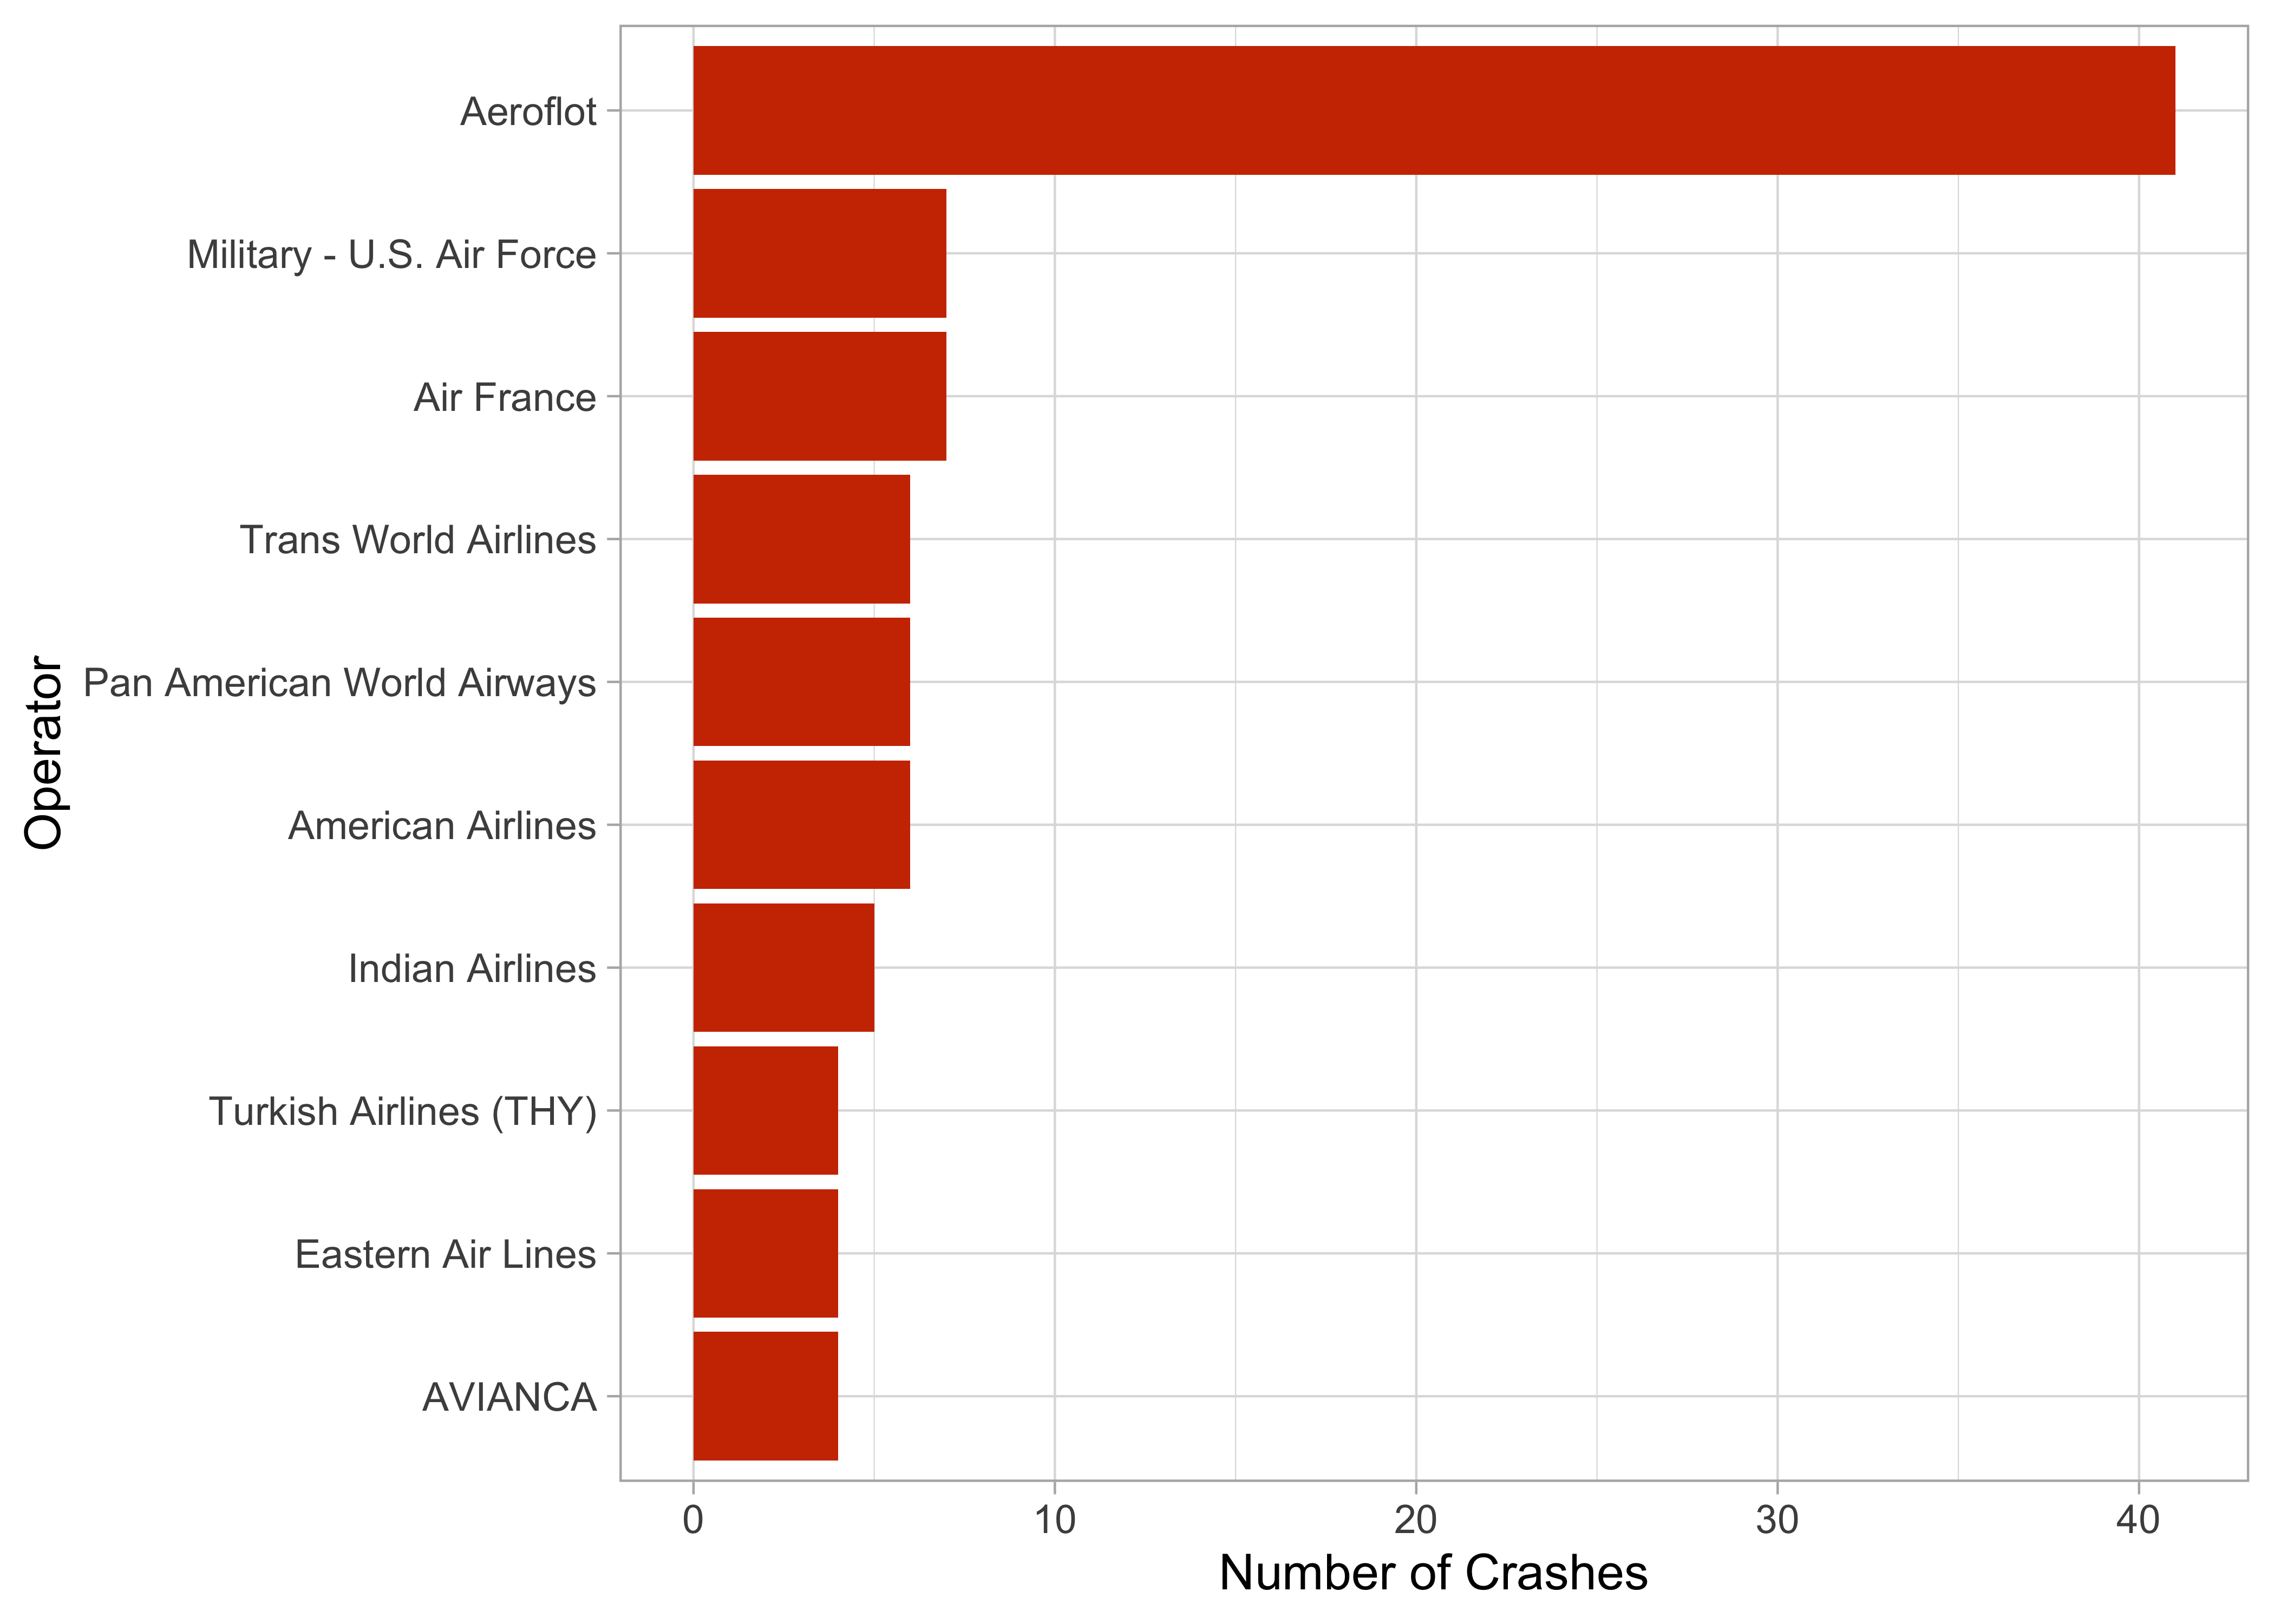
\includegraphics[width=0.46\textwidth]{Op2-1.png}}
\end{figure}
\begin{itemize}
    \item A wide mix of airlines make up the top ten list of large passenger plane crashes with high survival rates. 
    \item The Russian Aeroflot airline stands out as the top large passenger plane crashes with high fatalities. At over 40 deadly crashes on record, Aeroflot has 4 times more deadly crashes than any other operator on the top ten list of large passenger plane crashes with high fatalities. 
\end{itemize}
Russian airline Aeroflot and Russian aircraft models Tupolev and Ilyushin stand out among the top 10 list of large passenger plane crashes with high fatalities. This may be related to the weather and other conditions in Russia.
\subsection{Locations and Air Crashes}
We plotted the locations of large plane crashes on the map, as shown in Figure \ref{fig:maps}. \begin{figure}[htp]
    \centering
    \caption{Location of the crashes}
    \label{fig:maps}
    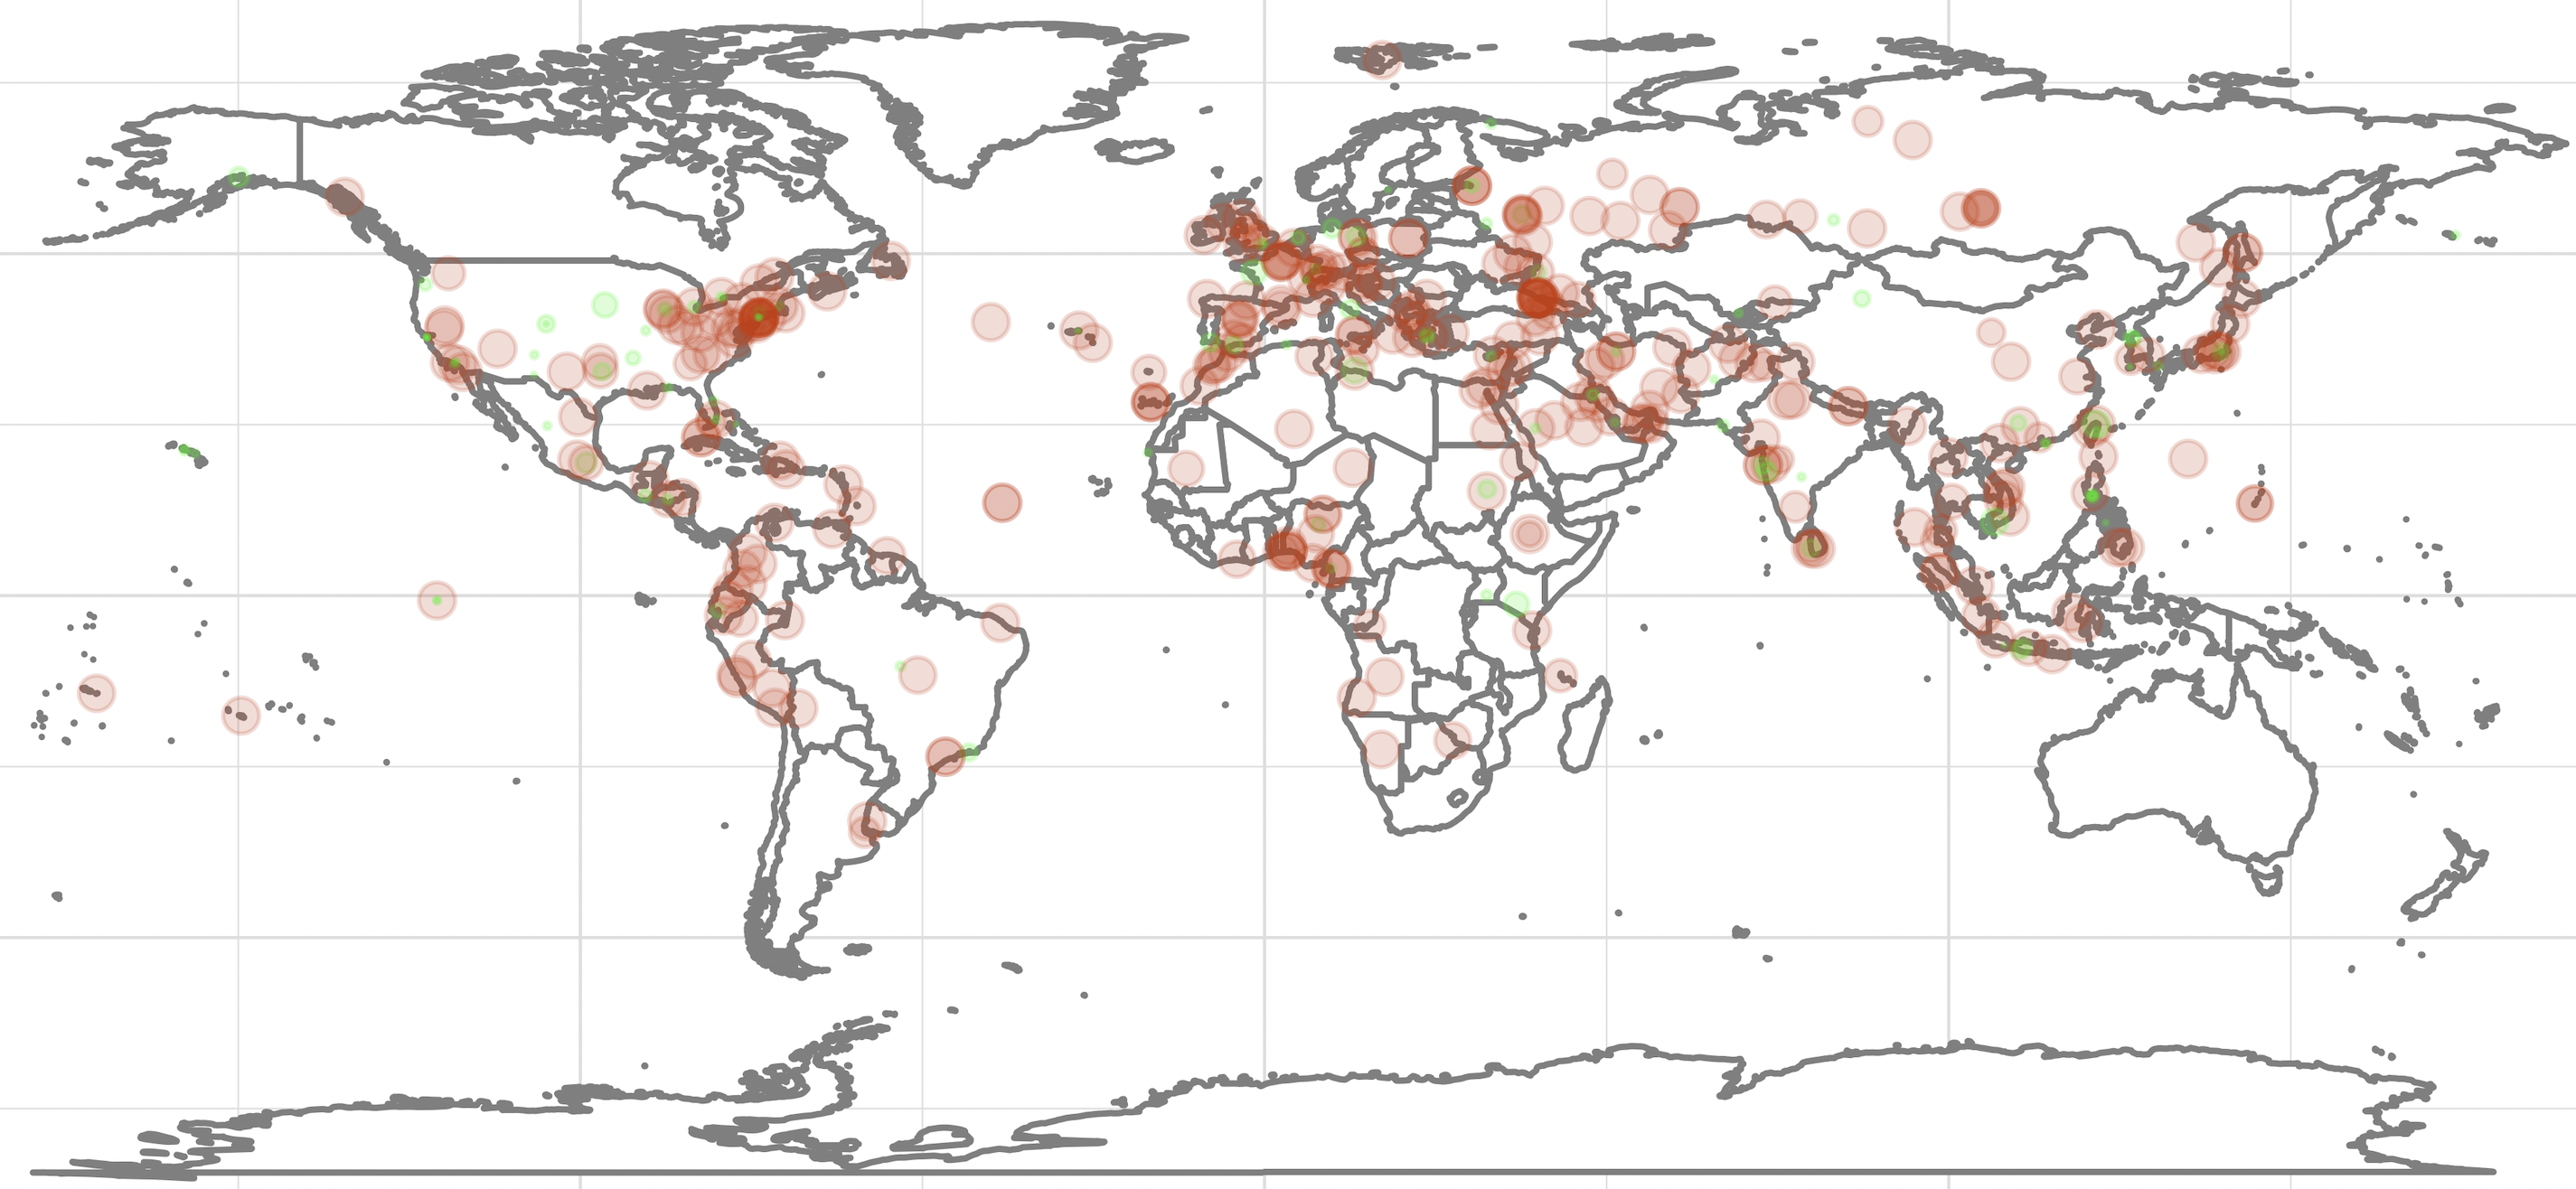
\includegraphics[width=.95\textwidth]{map-1.png}
\end{figure}
The red points in the map indicate high fatality crashes in which less than $30\%$ of passengers survived and green points represent high survival crashes in which greater than $65\%$ of passengers survived. The size of the points provide an indication of fatalities with larger points representing larger number of deaths. We can see the following two points from the plot. 
\begin{itemize}
    \item Majority of crash sites appear in the northern hemisphere. 
    \item Majority of crashes occur near the coast of countries of continents. 
\end{itemize}
\section{Conclusion}
Although we have analyzed many of the factors that contribute to the low survival rate in air crashes, the fact is that the fatalities in airplane crashes are much lower than the fatalities in other modes of transportation. 
To avoid low survival rates in crashes, we have the following suggestions.
\begin{itemize}
    \item Don't fly with Aeroflot, there is $68\%$ chance of you dying. 
    \item Don't fly in a Douglas DC-3, you are 5 times more probable to die. 
\end{itemize}
\end{document}